\documentclass[useAMS,usenatbib,tightenlines,11pt,preprint]{aastex}
%\documentclass[useAMS,usenatbib,tightenlines,11pt,preprint]{aastex}
\usepackage[paperwidth=8.5in,paperheight=11in,centering,margin=1in]{geometry}

\usepackage{parskip}
%\setlength{\parskip}{\baselineskip}
\parskip=5pt

\usepackage{amsmath}
\usepackage{amsbsy}

\input epsf
\usepackage{amsmath,amssymb,subfigure}
\usepackage{graphicx}
\usepackage{epsfig}
\usepackage{color}
%\usepackage{ulem}
%\usepackage{epstopdf}

\usepackage{multicol}
%\usepackage{etoolbox}

\pagestyle{empty}

\renewcommand{\baselinestretch}{0.99}

%%%%%%%%%%%%%%%%%%%%%%%%%%%%%%%%%%%%%%%%%%%%%%%%%%%%%%%%%%%%
%%%%%%%%%%%%%%%%%%%%%%%%%%%%%%%%%%%%%%%%%%%%%%%%%%%%%%%%%%%%
%%%%%%%%%%%%%%%%%%%%%%%%%%%%%%%%%%%%%%%%%%%%%%%%%%%%%%%%%%%%

\begin{document} 

\begin{center}
{\bf \Large Learning in an Era of Uncertainty}
\end{center}

\vspace{1cm}

\noindent
\begin{tabular}{ll}
{\bf Applicant/institution: } & University of Washington\\
{\bf Street Address: } & \\
{\bf Principal Investigator: } &Andrew Connolly \\
{\bf Telephone number: } & (206) 543 9541 \\
{\bf Email: } & ajc@astro.washington.edu \\
{\bf Administrative POC name:} & Lynnette Arias\\
{\bf Telephone number:} & 206-543-4043\\
{\bf Administrative POC name:} & osp@uw.edu\\
{\bf Funding Opportunity FOA Number:} & DE-FOA-0000918 \\
{\bf DOE/OSP Office: } & Office of Advanced Scientific Computing Research \\
{\bf DOE/Technical Contact: } & Dr. Alexandra Landsberg \\
{\bf PAMS Preproposal tracking number: } & PRE-0000002147 \\
\end{tabular}

% \noindent 
% \begin{tabular}{ll}
% {\bf Applicant/institution: } & Carnegie Mellon University \\
% {\bf Street Address: } & 5000 Forbes Ave, Pittsburgh, PA  15213 \\
% {\bf Co-Principal Investigator: } & Jeff Schneider \\
% {\bf Telephone number: } & (412) 268 2339 \\
% {\bf Email: } & schneide@cs.cmu.edu \\
% {\bf Administrative POC name, number, email:} Kristen Jackson, (412) 268 9527, kristenr@andrew.cmu.edu & \\
% {\bf Funding Opportunity FOA Number:} & DE-FOA-0000918 \\
% {\bf DOE/OSP Office: } & Office of Advanced Scientific Computing Research \\
% {\bf DOE/Technical Contact: } & Dr. Alexandra Landsberg \\
% {\bf PAMS Preproposal tracking number: } & PRE-0000002147 \\
% \end{tabular}

\newpage

{\bf Collaborating Institutions:} \\
Lead Institution: University of Washington, PI Andrew Connolly \\
Collaborating Institution: Carnegie Mellon University, PI Jeff Schneider \\

{\bf Lead PI:} Andrew Connolly \\

\noindent
\begin{tabular}{|l|l|l|r|r|r|r|}
\hline
\multicolumn{7}{|c|}{\bf Learning in an Era of Uncertainty} \\ \hline
&       &             & Year 1 & Year 2 & Year 3 & Total \\
& Names & Institution & Budget & Budget & Budget & Budget \\ \hline
Lead PI & Andrew Connolly & U Washington & \$170K & \$170K & \$170K & \$510K \\ \hline
Co-PI & Jeff Schneider & Carnegie Mellon U & \$170K & \$170K & \$170K & \$510K \\ \hline
{TOTALS} & & & \$340K & \$340K & \$340K & \$1020K \\ \hline
\end{tabular}

% \label{firstpage}

% \maketitle 
\pagebreak

%\begin{center}
%{\bf \Large Learning in an Era of Uncertainty}
%\end{center}

\section{Introduction}


A new generation of DOE sponsored data intensive experiments and surveys,
designed to address fundamental questions in physics, materials, and
biology will come on-line over the next decade. These experiments share
many similar challenges in the fields of statistics and machine-learning:
how do we choose the next experiment or observation to make in order that
we maximize our scientific returns; how do we identify anomalous sources
(that may be indicative of new events or potential systematics within our
experiments) from a continuous stream of data; how do we characterize and
classify correlations and events within data streams that are
inherently noisy and
incomplete. The goal of this proposal is to address these challenges
through the development of machine learning techniques that better quantify the
uncertainty in their predictions and corresponding active experiment
selection algorithms that utilize those uncertainties to get the most
scientific information out of limited data collection budgets.

{\it Active learning} algorithms iteratively decide which data
points they will collect outputs on and add to a training set.  Their
goal is to choose the points that will most improve the model being
learned.  At each step, they consider the current training data, the
potential data that might be obtained, and the current learned model,
and evaluate what would be the best choice for the next observation,
experiment, or feature such that it improves our knowledge of the
overall system (according to some objective criterion). The potential
impact of active learning algorithms is substantial (optimizing the
scientific returns from billion dollar investments in observational
facilities). To achieve these breakthroughs requires that we address
the challenge of how to scale active learning to the size and
complexity of the data expected from this next generation of
experiments.  For example, our inability to undertake a full look
ahead to the end of all possible experiments results in the
development of myopic heuristics that improve the speed of these
learning techniques but at a substantial cost in how well they perform
on real data.  See, for example, 
Figure 1 from Garnett {\it et al}. (2011) and Figures
3 and 4 of Garnett {\it et al}. (2012a).

By addressing these challenges we propose to develop active learning
algorithms that will scale to data sets with hundreds of millions of
entries and petabytes of data. This work has the potential to impact
many of the data intensive sciences. For this proposal, however, we
will focus our work in the context of DOE sponsored cosmology
experiments (i.e.\ the Dark Energy
Survey\footnote{http://www.darkenergysurvey.org}, and the Large
Synoptic Survey Telescope\footnote{http://www.lsst.org}). These
surveys are ideal proxies as their bandwidth (terabytes of data per
night and petabytes of data every couple of months) will enable high
precision studies of cosmology. The ability to use these data sets to
achieve an order of magnitude improvement in our constraints on our
understanding of cosmology and dark energy will, however, depend on
how well we can analyze, optimize, and calibrate data streams that are
noisy and incomplete. This requires developing
fundamentally new approaches to the analysis of data at a scale,
speed, and complexity beyond the capabilities of current automated
machine learning methods.

\subsection{Project Objectives}
\label{sec:objectives}

On-line, data-driven analysis will require model-fitting and
classifications that are non-parametric and probabilistic.  Gaussian
Processes meet these requirements and therefore we will build our methods
around them.  We note, however, that all the active experiment selection
algorithms we will develop will be applicable to any other alternative models that also
provide appropriate distributions with its predictions{\bf XXX not
  sure what this means}.  We divide our
research program into the following objectives.

{\bf Designing Robust Gaussian Processes.}  Figures \ref{fig:scatter}
and \ref{fig:lnsum} below will demonstrate that, ``out of the box,'' Gaussian
Processes can already perform much better than other algorithms (both
forward-fitting and data-driven) for model inference. Extending them
to the future of big-data science will, however, require confronting problems not yet
faced by automatic data analysis algorithms. {\it Model degeneracy} -- most model-fitting algorithms, including Gaussian
Processes, are written to return an optimal value (whether a latent physical
variable or a classification) and some error on that value.  This assumes that
the true model obeys single-mode Gaussian statistics.  As future experiments
continue to push the boundaries of our physical understanding, this assumption
will cease to be valid and we will be forced to build algorithms that can
accommodate multi-modal models obeying a wide range of probabilistic
distributions.  We propose a series of modifications that will allow Gaussian
Processes to function in this regime.
{\it Incomplete training data} -- the difficulty of experiments being attempted
in high energy physics, astrophysics, and biology often means that, not only is
the gathering of data expensive, it may not be possible in some regimes.  Future
algorithms will need to be able to make inferences about models in regimes where
training data is either very sparse not available at all.  Because of their
non-parametric design, Gaussian Processes are amenable to this kind of
modeling and we propose additional modifications that will enhance their
robustness against such incomplete training data.

{\bf Active Learning.} Supervised regression and classification algorithms
require labeled data points for training.  These output labels are obtained
through labeling by human experts and/or additional data collection.
Often, the resources required (both in terms of human-hours and
experimental apparatus) are considerable.  We propose to develop new
algorithms to optimize the use of these resources by determining what event
or object labels will maximize the improvement to models from supervised
learning algorithms.  Our preliminary implementation using a classical
heuristic on the problem of determing astronomical Doppler shifts (or
redshifts) from broad-band photometric data already shows the promise of
active learning in cosmology.  We propose novel algorithms based on new
myopic criteria and increasing the computational scalability of lookahead
methods that will greatly improve the accuracy and coverage of learned
models.

{\bf Active Feature Acquisition.}  Active Learning selects specific
unknown events or objects for follow-up observation and classification
by human experts.  Active Feature Acquisition further refines our
inquiry by asking what kinds of follow-up observations will yield the
most information about the unknown object.  We propose to extend our
recent work on using Gaussian Processes (GPs) to detect damped
lyman-alpha (DLA) systems \cite{Garnett12a}.  In that work GP
regression was used on each observed, noisy spectrum to infer the
latent spectrum.  The single independent (input) variable was
wavelength.  In other problems (such as the identification of
astronomical transients) there will be several input variables which
we can choose to observe or ignore.  
We will build an information-theoretical framework to make this choice.
In the DLA work, a binary choice was made between models with and
without a DLA.  DLAs were
classified by recognizing which model fit best.  In the proposed work,
we will learn a different model for each class of object and will
estimate class probabilities using Bayes rule for combining the prior
probability for each class and how well the respective models fit the
observations.  We will apply these techniques to the challenge of
characterizing and classifying the light curves of supernovae (used in measuring the
cosmic acceleration) from data with poor temporal sampling,
%increasing the number of supernovae that can be used for cosmological
%experiments by an order of magnitude.  
The key advantage of this
approach is that the GPs naturally provide a mean and covariance for
future unobserved observations (see Section \ref{sec:gp} for a more detailed
discussion).  This uncertainty propagates through
to class labels and we can use it to estimate the reduction in class
uncertainty that will be gained by making a given observation at a
specific time.  The observation yielding the greatest reduction in
entropy for the class and the light curves for this object will be
taken.

{\bf Active Search.} Often it is the anomalous events within large
streams of data that lead to fundamental breakthroughs. We, therefore, require
methods for
rapidly identifying and classifying potentially novel events and objects
while staying within the limited budget of additional experiments that
might be undertaken to confirm these discoveries.
This is an active search problem. The
problem and the Bayesian optimal algorithm for it are described in our
recent work \cite{Garnett11,Garnett12}.  As in active learning, the
acquisition of class labels is expensive and we need to learn a model to
predict these labels from limited input data. The final
performance objective is, however, not the accuracy of the classifier, but rather the
number of positives (i.e. objects from interesting classes)
identified. Our previous work considered a binary classification problem: ``is
the object `interesting' or not?''  We will extend this work to allow for
classification according to a continuous scalar function or multiple discrete
classes.  We will design algorithms that consider probability distributions
across all possible classes and
quantify how new observations will affect these
distributions with an eye towards reducing the entropy, or some other
information-theoretical measure of uncertainty.

% We
%propose to use the simple myopic algorithm described in that work.  It
%computes the probability of each point belonging to the positive class and
%chooses the largest.



%The active search and active learning algorithms each compute an objective
%criterion score for each object.  For photometric redshifts the scores are
%used to create a ranked list and observations are scheduled proceeding down
%the list.  When a budget is given for follow-ups on each batch of newly
%detected transients, going down a ranked list in each batch until that
%budget is exhausted is appropriate.

%However, when the budget is an aggregate over a longer time period a
%streaming decision on how much of the budget to spend on each batch must be
%made on that batch in isolation.  This will be done by choosing a score
%threshold.  The threshold will be set by evaluating the historical stream
%and setting it at a value that would yield a number of follow ups equal to
%an available budget for following up.  The threshold will be adjusted
%continuously as more observations are taken and the models and scientific
%goals change (e.g. the object types designated as ``interesting'' are
%changed).

{\bf Science Outcomes.}  Data from the Dark Energy Survey will become
publicly available over the term of this project (together with
detailed simulations of the expected data flow from the LSST).  We
will, therefore, use these data to demonstrate
that the algorithms developed above will improve the cosmological
reach of the DES and LSST in the areas of  
improved determination of photometric
redshifts (see Section \ref{sec:photoz}) and improved classification and online
follow-up of transient astronomical objects.  We will release our software
publicly and seek collaborations where our algorithms may be spread to
other sciences -- such as climatology and microbiology -- wherein complex
systems can be modeled or measured at great expense and algorithms are
required to determine which models and experiments are actually worth
performing.

Each of these goals will require us to develop algorithms to simultaneously
learn the latent physical model underlying a given data set, the
uncertainties around that model, and the potential information to be gained
by futher studying a specific instance of the model (``event'' or
``object'').

\subsection{The Collaboration}

To accomplish the objectives laid out in this program we have
assembled a team experienced in algorithm design, data structures, and
in developing and delivering data mining algorithms that are actively
used by the cosmology community. The PIs of this research proposal
have a proven track record for propagating research ideas in
educational and multidisciplinary environments. Connolly and Schneider
have been part of an ongoing collaboration between machine learning,
cosmology and statistics for over a decade (noted by the President
of the American Statistical Association (ASA) as an exemplary
interdisciplinary research team \cite{straf03}).

Highlights from this collaboration include n-tree searching algorithms
that make the calculation of n-point correlation functions scale to
the size of current surveys \cite{GrayMoore} and that enable rapid
characterization of orbital tracks in sparsely sampled temporal data
\cite{kubica}. The software associated with these algorithms was made
publicly available and has been used to compute the 2--point function
on over 10$^6$ galaxies and the 3--point correlation function of
400,000 galaxies from the SDSS survey
\cite{Scranton2002,Szapudi2002,Nichol2006,mcbride2011a,mcbride2011b}
as well as in measures of the marked correlation functions
\cite{Skibba2006}.  As part of this collaboration \citet{yip2004a,
  vdp2009, daniel2011} introduced, to astrophysics, signal compression
and analysis techniques that are now regularly applied to the analysis
of spectroscopic surveys. More recently this collaboration has
developed algorithms for automatically classifying astronomical objects
\cite{vdp2009,daniel2011} as well as an initial set of papers that use
a simplified active learning method to accelerate the exploration of
complex parameter spaces \cite{daniel2012}.  Schneider's group has led
the development of several new methods of regularization to learn
complex models with only a small amount of training data
\cite{YiZhangICML2010,YiZhangSDM2010,YiZhangMultitask2010,YiZhang2011multiECOC,YiZhang2012},
for non-parametric estimators for divergences and dependencies
\cite{poczos11alphadiv,Poczos2011UAI,poczos12CVPR}, and for graphical
models for finding groups of collectively anomalous records
\cite{Xiong2011gad,xiong2011fgm}.
 
Connolly leads the University of Washington data management group that
develops the algorithms and techniques for the real-time analysis of
LSST data (including the detection and characterization of
transients and anomalies).  Schneider heads a machine learning group
that has done extensive work on automatic anomaly detection and
pattern-recognition in complex data sets
\cite{Xiong2011gad,poczos12CVPR}.  Schneider, and Connolly are members
of the Large Synoptic Survey Telescope collaboration with Connolly the
software coordinator for the DOE sponsored Dark Energy Science
Collaboration (a collaboration of over 150 scientists working on the
characterization of dark energy).


On the educational front, all PIs have developed and taught computational techniques at the
graduate and undergraduate level including data-mining for
Astrophysics. Connolly recently completed a text book ``Statistics,
Data Mining, and Machine Learning in Astronomy: A Practical Python
Guide for the Analysis of Survey Data'' that will be published by
Princeton University Press and provides a comprehensive introduction
to cutting-edge statistical methods together with the software
associated with these techniques. On sabbatical at Google, Connolly led the
development of Sky in Google Earth (aka Google Sky;
http://earth.google.com/sky), which was similarly successful at
engaging the public.

%We expect the proposed research to move beyond astrophysics to other
%data intensive sciences. In its broadest sense machine learning for
%massive Petabyte data archives drives many of the physical and
%biological sciences with catalogs containing hundreds millions of
%samples with thousands of measurements. The algorithms to be
%investigated here will also impact machine learning beyond their
%application to cosmology.  They move beyond the traditional learning
%of full models and are able to handle data that do not need to be
%pre-assembled into temporal sequences.  If successful, this will add
%new types of data sets and by inference new scientific fields to the
%list that can benefit from active learning of models.

\section{The Role of Active Learning in Cosmology}

Over the last decade a concordance model has emerged for the universe
that describes its energy content. The most significant contribution
to the energy budget today comes in the form of ``dark energy'', which
explains the observation that we reside in an accelerating
universe. Despite its importance to the formation and evolution of the
universe there is no compelling theory that explains the energy
density nor the properties of the dark energy. Understanding the
nature of dark energy remains as one of the most fundamental questions
in Physics today, impacting our understanding of cosmology, particle
physics, and potentially theories of gravity itself.  As noted in the 
report of the Dark Energy Task Force (DETF; constituted jointly by
DOE, NSF and NASA), ``the nature of dark energy ranks among the very
most compelling of all outstanding problems in physical science''.


To address the question of the nature of dark energy a new generation
of DOE sponsored experiments are entering service (e.g.\ the Dark
Energy Survey and the
Large Synoptic Survey Telescope).  These
surveys will represent a 40-fold increase in data rates over current
experiments (generating over 100 Petabytes of data over a period of 10
years) and decreasing the uncertainties on our measures of the
underlying properties of dark energy by more than a factor of ten.


At the scale of these experiment, statistical noise will no longer
determine the accuracy
 to which we can measure cosmological
parameters. The control and
 correction of systematics will
ultimately determine our final
 figure-of-merit. For example,
systematic errors in the estimation of cosmological distance or in the
identification and classification of high energy transient events
(e.g. supernovae) lead to biases in the derived cosmological
parameters. A bias of 1\% in distance (at a redshift $z=1$) degrades
measures of the properties of dark energy by over 50\%
\cite{kitching,huterer2006,nakajima2011}.

%\subsection{orphaned paragraphs about the importance of our science cases}
%
%The accurate determination of an object's distance or redshift is
%central to every test of cosmology that happens outside of a particle
%accelerator.  The comparison of redshifts and luminosities of standard
%candles enabled the discovery of dark energy and cosmic acceleration
%\cite{perlmutter1998}. Redshifts serve as a proxy for radial distance
%from Earth to the observed object.  Redshifts thus are necessary for
%building three dimensional maps of the distribution of galaxies in the
%Universe.  Such maps will help and have helped us to constrain how
%galaxies formed over the history of the Universe, and thus can tell us
%much about how gravity operates at the largest scales and what the
%parameters are that govern the behavior of dark energy, dark matter, 
%and the cosmic
%acceleration \cite{muvarpi2,roland,sudeep,linder2013}.  Accurately determining the redshifts of
%distant galaxies is a requirement if we are to answer some of the most
%vexing problems in fundamental physics today.
%
%Direct spectroscopic redshift measurements of enough galaxies to
%constrain dark energy parameters to the precision required by next
%generation experiments would be thousands of times more expensive than
%taking the corresponding photometric (or imaging) data.  Large digital
%cameras (e.g.\ the 3.2 Gigapixel camera for the LSST) can observe
%$\sim 10^6$ sources every 15 seconds (several orders of magnitude more
%efficient that spectroscopic observations). Our task, then, is to
%construct algorithms whereby we can convert these much cheaper
%photometric data into accurate redshifts (i.e. photometric redshifts).
%
%The demands of next generation cosmological experiments will require
%that our photometric redshift determinations be accurate to within
%$\le 2\times 10^{-3}(1+z)$ \cite{desc}.  This is a hard limit, as a
%bias in redshift determination of just 0.01 can degrade dark energy
%constraints by as much as 50\%
%\cite{kitching,huterer2006,nakajima2011}.  Testing present forward-fitting
%and empirical methods on a sample of 5,482 galaxies from the 2df-SDSS
%LRG and Quasar survey, Abdalla {\it et al}. (2011) find biases of
%order 0.05 (see their Figure 4).  This level of bias can degrade dark
%energy constraints by as much as a factor of 3 \cite{Ma2006}.
%Considering 3,000 galaxies from the DEEP2 EGS and zCOSMOS surveys and
%using Bayesian methods, Mandelbaum {\it et al}.  (2008) find a bias in
%redshift determination of order 0.01 (see their Table 2).  While this
%is an improvement, it still an order of magnitude larger than what is
%required.
%

\section{A Probabilistic Framework for Scientific Inference}

Current state-of-the art algorithms attempt to learn a 
model as a one-to-one
relationship between the input data and the output function. Uncertainties are
also learned, but these are usually heuristics derived by considering multiple
attempts at model-fitting such as by a committee of aritficial neural networks
\cite{annz}.  We propose to replace this framework with one that directly models
the probability distributions underlying the data.
We believe that this framework
is the most robust and informative available.  It will allow us
to learn, not only
the models underlying the data, but the uncertainties surrounding these models,
and the potential information to be gained from different follow-up
observations.  These three inferences will be critical in an age of
research with low tolerance for uncertainty and limited budgets for
follow-up observation and will allow us to extend our algorithms' application
beyond realm of function regression and into that of object classification.
We will build this new framework on the foundation of Gaussian Processes.  

\subsection{Gaussian Processes}
\label{sec:gp}


Gaussian processes (GPs) model the output of an unknown, noisy function
in multi-dimensional data space
such that any set of samples from it has a joint multivariate Gaussian
distribution \cite{gp}.  Given a set of observed samples from the function's
data space, a GP
can make predictions about a set of other locations and assign these
predictions a multivariate Gaussian distribution.  An important
feature of GPs is that they do not make parametric assumptions about the
form of the function they are modeling and thus are well suited to
nonlinear regression problems.

GPs have been used successfully to describe a wide range of physical
phenomena without having to assume a model of the underlying process, even
in the case of sparse measurements.  Examples in astrophysics include the
expansion history of the universe \cite{ericgp} and interpolating point
spread functions across large images \cite{psf}.  Mahabal {\it et al}. (2008b) 
and Wang {\it et al}. (2011,
2012) use a mixture of Gaussian Processes to model light curves and
identify periodically varying stars.  Huisje {\it et al}. (2011, 2012)
improve upon their methods, using information-theoretical quantities to
separate the true period of these variations from systematics introduced by
observational apparatus.  The PIs have used GPs to accelerate the search of
high-dimensional likelihood functions on the cosmological parameters by
efficiently selecting sample points \cite{daniel2012}, to detect damped Lyman
alpha systems in the spectra of quasars \cite{Garnett12a}, and to optimize the
performance of complex robots \cite{Tesch11a,Tesch11b,Tesch13}.

We now describe how the underlying function is modeled with a GP based on a
sample of training data.  Assume that each training set datum is of the
form $\{\vec{\theta},y\}$, where $\vec{\theta}$ is an $N_p$-dimensional
vector representing the measured data (input) and $y = f(\theta)$ is the
latent quantity (output) we are trying to infer.  $f$ is assumed to be a
probabilistic function on the $N_p$-dimensional space with some covariance
function relating pairs of points on the function, such as a squared
exponential covariance,
\begin{equation}
\label{eq:covariogram}
K_{ij}\equiv\text{Cov}\left[f(\vec{\theta}_{i}),f(\vec{\theta}_{j})\right]
= \exp(-\frac{1}{2}|\vec{\theta}_{i} - \vec{\theta}_{j}|^2/\ell^2)
\end{equation}
where $\ell$
is a characteristic length scale set by cross-validation.  
Under those
assumptions, one can derive a posterior probability distribution for $f$
at a new query point $\{\vec{\theta}_{q}\}$ by marginalizing over
the measured points $\{\vec{\theta}\}$.  This gives a Gaussian distribution
with mean:

\begin{equation}
f(\vec{\theta}_q)=\bar{y}+K_q\left(K+\sigma^2 I\right)^{-1}(\vec{y}-\bar{y})
\label{eq:mean}
\end{equation}

\noindent
and variance:

\begin{equation}
\Sigma_{q} = \text{Cov}(f_{q}) = K_{qq} - K_q^T (K + \sigma^2I)^{-1} K_q
\label{eq:cov}
\end{equation}

\noindent
Here, $K$ is the matrix of
covariances between all training points, $\sigma^2$ is the variance of
Gaussian noise added to each observed value of $y$, $\vec{y}$
is the training data outputs, $\bar{y}$ is the algebraic mean of the elements of
$\vec{y}$, and
$K_q$ is the vector of covariances between the query point and all
training points.  Eq.~\ref{eq:cov} extends directly to the case of multiple
query points by taking the variables as matrices where appropriate, and the
result is a full covariance matrix for the query points.  Readers looking
for a more detailed explanation of GPs should consult
Rasmussen and Williams (2006).


The inferences in equations \ref{eq:mean} and \ref{eq:cov} are non-parametric:
they do not assume a form for the latent model they represent.  This makes GPs
especially powerful at learning models over data
with complex degeneracies.  We demonstrate this with the following problem.

\subsection{Photometric redshifts: a Gaussian Process case study}
\label{sec:photoz}

One science use case for the algorithms proposed here is the problem of learning
photometric redshifts.  Any attempt to solve the astrophysical problem of dark
energy requires measuring the cosmological Doppler shift of light from hundreds of
millions of galaxies.  Directly measuring the spectra of these galaxies is
prohibitively expensive.  Measuring their brightness in a handful of broadband
filters (i.e., taking their photometry), is several thousand times cheaper. 
For this reason, surveys such as the DES and the LSST are designed to exclusively take
photometric data and rely on algorithmic researchers to deliver ways
of inferring a relationship between a galaxy's observed photometry (usually in five or
six bands) and it's true redshift.

Photometric redshifts are principally determined using
forward-fitting models.  Astronomers assume that they can model the rest frame
spectra of any galaxy.  These spectral models are
redshifted and integrated over the profile of an experiment's
photometric filters until a good fit to the observed photometric data is
found.  The redshift of the galaxy is taken as that which produces the best fit
between model and data.  Many publicly available codes such as 
EAZY \cite{eazy} implement this method.  
While it is straightforward in principle, it requires
accurate foreknowledge to select the appropriate rest frame 
spectral models.  If the chosen
models are not representative of the population of observed
galaxies, the algorithm will fail to give accurate redshifts and cosmological
inferences will be inaccurate \cite{budavari2008}.  The effects of this
shortcoming can be seen in Figure \ref{subfig:eazy}, which plots the results
of running EAZY on a set of
simulated galaxy observations designed to represent data expected from the
LSST.
While many of the galaxies fall near the
$z_\text{photometric}=z_\text{spectroscopic}$ line, there is significant scatter
in the results.  Figure \ref{subfig:gp} plots the results from running the same
simulated galaxies through GP-based algorithm that attempts to learn the full
probability distribution $P(z_\text{photometric})$.  There is much less scatter
in this case than in the case of the forward-fitting modeling of EAZY.

\begin{figure}[th]
\subfigure[]{
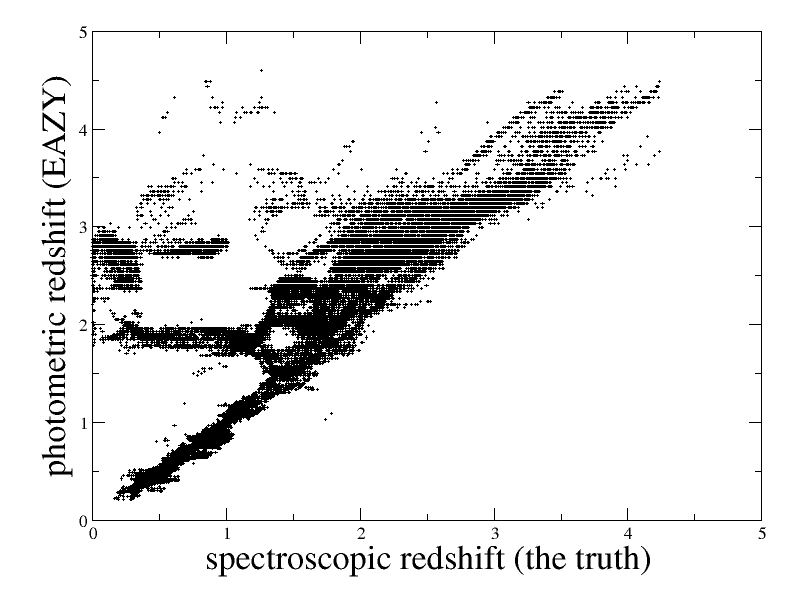
\includegraphics[scale=0.3]{eazy_scatter_plot.png}
\label{subfig:eazy}
}
\subfigure[]{
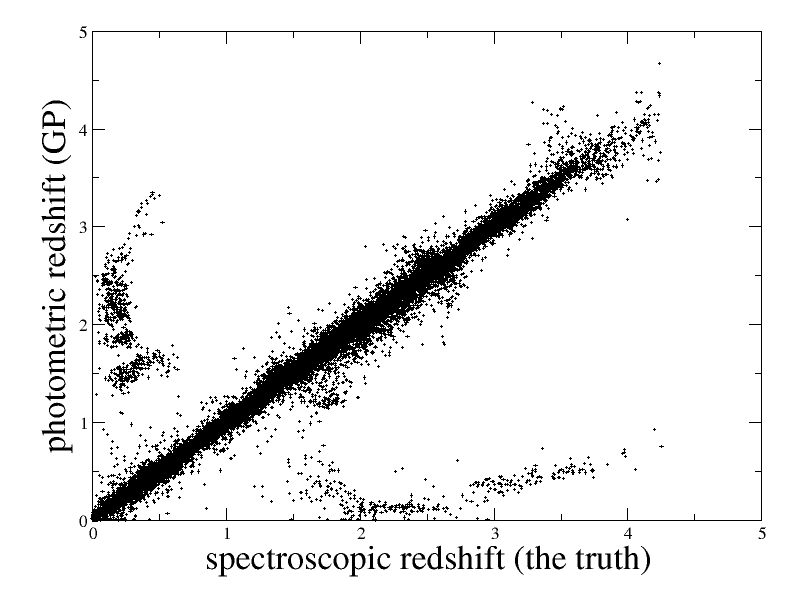
\includegraphics[scale=0.3]{gp_scatter_plot.png}
\label{subfig:gp}
}
\caption{
Photometric redshift plotted
against true spectroscopic redshift for 48,000 simulated LSST galaxy
observations.  Photometric redshifts are derived using the
EAZY template-fitting
algorithm (a forward model) in Figure \ref{subfig:eazy} and
our GP based algorithm in Figure \ref{subfig:gp}.
}
\label{fig:scatter}
\end{figure}

Other data-driven algorithms for photometric redshift determination do exist. 
An example of these is the publically-available code ANNz \cite{annz},
which is based on an artificial neural network scheme.
In this case, the principal
shortcoming the method is that the artificial neural network
is designed only to return only a
photometric redshift value and an uncertainty.
This uncertainty is a heuristic combination of the uncertainties in the
photometric data as well as the scatter in $z_\text{photometric}$ derived
from multiple instantiations of ANNz.  There is no guarantee that it represents
the true, probabilistic uncertainty in $z_\text{photometric}$.
Figure \ref{fig:lnsum} plots the mean value of $\ln[P(\text{truth})]$,
i.e. the value of the logarithm $P(z_\text{photometric})$ at the point
$z_\text{photometric}=z_\text{spectroscopic}$, 
as a function
of photometric redshift for EAZY, ANNz, and our GP algorithm.
We see that both EAZY and ANNz consistently assign lower probabilities to
$z_\text{photometric}=z_\text{spectroscopic}$ than does our GP algorithm.

Other works have attempted to apply GPs to the problem of
photometric redshfifts \cite{kaufman,bonfield}, however, they have treated
the problem as one of learning the form of a one-to-one scalar function.
We propose to use the probabilistic nature of GPs to learn the full
probability distribution that a given galaxy is at a given redshift.  The
resulting prediction is simultaneously more robust against sparse, noisy or
degenerate training data, more usable in follow-on scientific analyses, and
more amenable to model improvement by the introduction of active learning.
% Figure \ref{subfig:gp} shows preliminary results from our algorithm when
% trained on spectroscopic data from 50,000 galaxies and tested on the same
% 48,000 galaxies as Figure \ref{subfig:eazy}.  Here we see that the GP
% modeling yields significantly less scatter about the true
% $z_\text{photometric}=z_\text{spectroscopic}$ relationship.

\begin{figure}[th]
\centerline{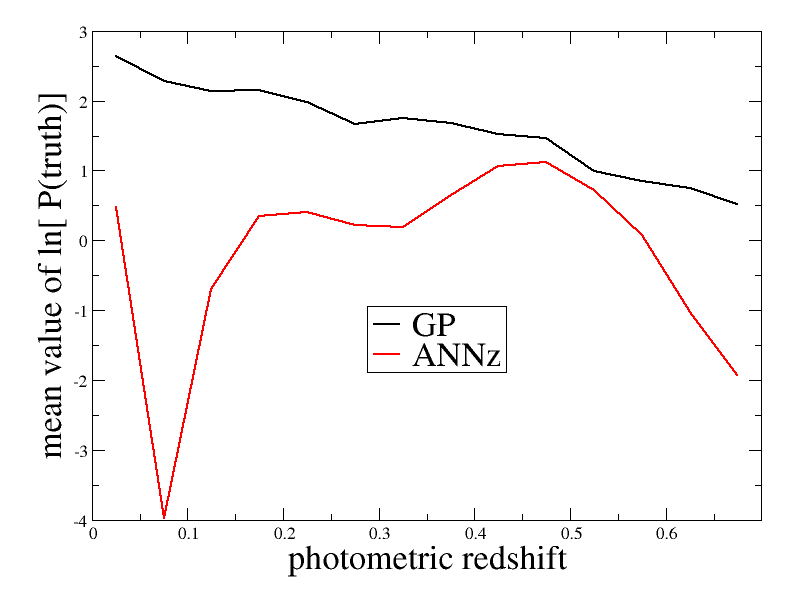
\includegraphics[scale=0.3]{sdss_lnsum.png}}
\caption{
The mean value of
$\ln[P(\text{truth})]$ as a function of photometric redshift (the vertical
axes in Figures \ref{fig:scatter}) for all
three algorithms under consideration using real
data taken from the Sloan Digital Sky Survey \cite{Abazajian:2008wr}.  
In this latter case, the
algorithms are trained on 21,000 galaxies and tested on 191,000 galaxies.
}
\label{fig:lnsum}
\end{figure}

The tests considered above represent idealized cases.
The algorithm resulting in Figure \ref{fig:scatter} was trained on high
signal-to-noise data with a training set sampled everywhere in
$z_\text{spectroscopic}$-space.  The algorithm resulting in Figure
\ref{fig:lnsum} is well-behaved in that the low redshift regime considered
exhibits no degeneracies in the photometry-to-redshift relationship.  This will
not be the case for the large, deep surveys of the future.  In order to extend
the favorable results of GPs above, further development of the
framework will be required.

\subsection{Fortifying Gaussian Processes against incomplete training data}

GPs are already designed to handle input data that is sparsely
sampled.  Equation \ref{eq:cov} gives the GP the freedom to declare a large
uncertainty in regions of data space where there is no training data.  However,
in order to deliver on the science results required by DES, LSST, and other
big-data surveys, it is not enough that $\Sigma_q$ be large where the model is
uncertain.  We require that $f_q$ in equation \ref{eq:mean} bear some
resemblance to the true answer {\bf XXX what does this mean}.  We propose to achieve this in several ways.
{\bf XXX for the bits below can you say in words what K$_{ij}$, theta, l etc
  mean - e.g. This assumes that the GP for all parameters ($\theta$)...} 

\begin{itemize}
\item New mean function models -- as presented,
equation \ref{eq:mean} set the value of $\bar{y}$ to the algebraic mean of the
training outputs $\vec{y}$.  This assumes that the GP for all $\vec{\theta}_q$
start from the same value from which equation \ref{eq:mean} encodes the
departures.  We will evaluate models more complex than the algebraic
mean but simpler than the GP, which can be used to give a more informative value
for $\bar{y}$ such that it interpolates over gaps in the training data.  We propose
to experiment with such functions, attempting to find a more robust foundation off
of which to build our GPs.
{\bf XXX do you have an example of one such function?}


\item Dynamic hyper parameters -- the value of $\ell$ in $K_{ij}$ is presented
as a parameter to be optimized by cross-validation.  This, again, selects a
single value for $\ell$ for all possible $\vec{\theta}_q$, regardless of
$\vec{\theta}_q$'s position in the data space.  We will develop 
dynamic algorithms, based on {\bf XXX ??}  for setting $\ell$ so that highly-sampled training data will
return small $\ell$ (tightly coupling the GP to the training data) and
sparsely-sampled training data will give larger $\ell$, allowing for broader
interpolation across gaps in the training data.

\item Learned $K_{ij}$ -- in the above discussion, the functional form of
$K_{ij}$ in equation \ref{eq:covariogram}
was assumed.  While this certainly resulted in acceptable behavior in
our test cases, it is by no means guaranteed that the choice we made (a Gaussian
function in data space) will always be the best choice.  We will introduce
algorithms {\bf XXX such as?} to help the GP learn the most appropriate form of the covariogram
based on the training data at hand, especially its distribution over the data
space.
\end{itemize}

\subsection{Fortifying Gaussian Processes against degenerate training data}

Additionally, it will be necessary to build GPs that are robust against the
possibility that degeneracies exist in the relationship between input and output
data.  This pitfall can already be seen in the simulated photometric redshifts
plotted in Figure \ref{subfig:gp}.  Note the high
$z_\text{spectroscopic}$ galaxies that appear at low $z_\text{photometric}$ and
vice-versa.  To correct for this error, we will harness the full probabilistic
nature of GPs, building a system which tests the simplest, single-mode Gaussian
model against multi-modal models.  The proposed algorithm will work as follows:
\begin{enumerate}
\item Fit the training data to a single-mode GP.

\item Use Bayesian model selection \cite{mackay}
to compute the model likelihood of this single-mode GP.

\item Divide the training data into two sub-populations based on their output
values.

\item Fit each sub-population to its own GP.

\item Compute the model likelihood of this two-mode model and compare to the
model likelihood of the single-mode model.

\item Repeat steps 3-5 for three-mode, four-mode, etc. models until
satisfied that you have found the best fit to the training data.
\end{enumerate}
Through this iterative approach, we expect to build a GP such that, even when it
succumbs to the degeneracies seen in Figure \ref{subfig:gp}, it will still place
significant probability density at the true
$z_\text{photometric}=z_\text{spectroscopic}$ value.  This will represent a
signtificant improvement over current model-learning algorithms, which are
principally concerned with returning a learned value for the model function and
some heuristic estimate for the uncertainty (i.e. neural networks).

\section{Active Learning}

A generic active learning algorithm takes the following form:

\begin{enumerate}

\item Learn a model (e.g. a Gaussian process) using the current set of
  labeled training data.

\item Evaluate the set or space of unlabeled data according to some active
  learning criterion, usually beginning by requesting the predictive
  distribution from the learned model.

\item Choose the data point/experiment with the highest evaluation and
  obtain the label for it (e.g. by requesting a data collection experiment
  and/or asking a human expert to provide the label).

\item Add the resulting data to the training data and repeat.

\end{enumerate}

The performance of an active learning algorithm is evaluated by some
measure of the model's quality (e.g. accuracy or log-likelihood on a test
set of data) as a function of the number of data points collected for the
training set.  The key algorithmic components are the model used in step 1
and the selection criterion used in step 2.  The previous section proposed
work on improving GP models.  In this section we propose new selection
criteria.

%We discuss specifically how we model $P(z_\text{photometric})$ below.

%Galaxy observations are represented as vectors $\{\vec{\theta}_q\}$ of
%flux information.  For each unknown
%test galaxy $\{\vec{\theta}_q\}$, we find the $k$ nearest neighbor training
%galaxies in flux space ($k$ is treated as a parameter to be optimized by our
%algorithm).  We divide these neighbor galaxies into two sub-populations based on
%their spectroscopic redshifts and fit a Gaussian Process to each sub-population.
%This gives us a bi-modal probability distribution for $P(z_\text{photometric})$. 
%We compare the likelihood of this hypothesis to a single-mode
%$P(z_\text{photometric})$ in which all of the neighbor galaxies are fit together
%in one Gaussian Process.  The final $P(z_\text{photometric})$ is a linear
%combination of these two hypotheses, weighted according to their respective
%model likelihoods.

\subsection{Novel active learning criteria}

\begin{figure}[t]
\centerline{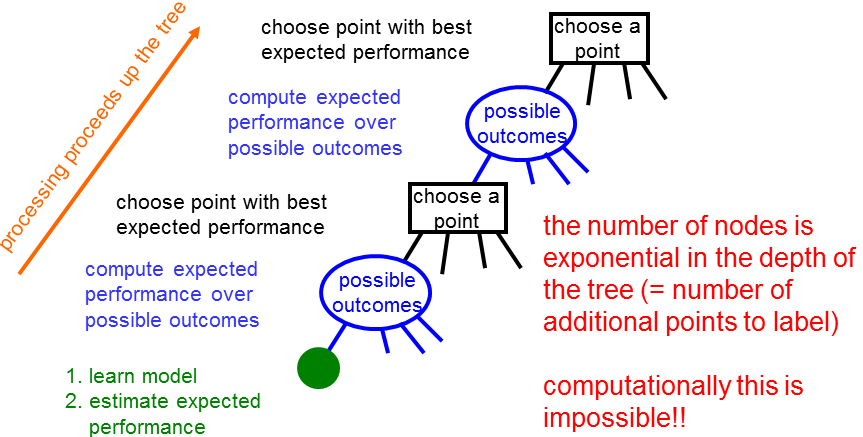
\includegraphics[scale=0.4]{searchtree.png}}
\caption{The search tree for an optimal active learning algorithm that will
  be allowed to choose two more data points.}
\label{fig:searchtree}
\end{figure}

It is useful to see the challenges involved in developing good active
learning criteria by considering what an optimal algorithm might need to
do.  Figure \ref{fig:searchtree} shows the computation it would require.
The root of the tree contains the current decision on which point to choose
and an optimal algorithm would consider them all.  For each choice, it
would then consider every possible outcome (label) that might be obtained
and weight them by the estimated probability of each outcome.  For each
outcome, it would then consider what next point it would choose if it
received that outcome.  The tree expands down to a depth equal to the
number of data points that will be chosen and at the leaf every possible
model would be learned and evaluated.  Since the number of leaves is
exponential in the depth of the tree, this quickly become intractable.  A
typical solution (referred to as myopic) is to truncate the tree to zero or
one level.  A second speedup is often obtained by replacing a full model
evaluation with a fast heuristic (see \cite{Settles09} for a summary of
common heuristics).

The evaluation of the model, whether in a full or truncated tree, is also a
challenge.  If we knew the true labels in our test set, we could use them
to evaluate the accuracy or log-likelihood of the true labels.  In a
simulated problem this is possible, but in a real application we do not
have the labels.  The usual alternative is to consider the uncertainty in
the predictions on the test points.  In the case of basic GPs, the
distribution is a multivariate Gaussian with covariance $\Sigma_q$ from
equation \ref{eq:cov} and the query is the entire test set.

A myopic information gain (change in entropy) strategy looks ahead one step
and chooses the data point that minimizes the expected entropy (monotonic
in $\det(\Sigma_q)$).  Even this can be expensive since it requires the
computation of the determinant.  An alternative is minimizing the average
variance ($tr(\Sigma_q)$, also known as V-optimality).  A further
approximation is to do no look ahead and simply choose the data point
corresponding to the largest diagonal element in $tr(\Sigma_q)$.  This is
known as uncertainty sampling.

We propose the following new methods:

\begin{itemize}

\item The usual implementations of the criteria listed above are based on
  Gaussian predictive distributions which means only the covariance need be
  considered.  We will develop efficient ways to estimate these quantities
  from our improved models of non-Guassian distributions.

\item Our preliminary experiments on classification in graphs indicate that
  the sum of all entries in the covariance matrix is a better criterion
  than the trace \cite{YifeiMa12}.  We propose to develop an analogous
  criterion for euclidean spaces and for regression problems.  This
  criterion has not been previously proposed in the experiment design
  literature and we will also analyze theoretically when and why it
  outperforms the alternatives.

\item It is clear that we can improve performance by looking ahead further
  (e.g. see \cite{Garnett12}).  We propose to develop pruning rules that
  will allow us to look ahead further using our improved models.  The rules
  will have the ability to trade off the aggressiveness of pruning, and
  thus the amount of look ahead allowed, against the approximation
  accuracy.  We will investigate when the additional look ahead allowed
  more than compensates for the errors induced by pruning.

\end{itemize}

% We will expand upon
% our recent work on the problem of optimal surveying or polling
% (Garnett et al 2012a).  Rather than having a goal of correctly
% predicting the output for each point in a test set, the goal is to
% predict the average output (or the class proportions in classification
% problems) over the test set.  This dramatically increases the
% efficiency of the active learning.  In preliminary experiments on
% graphs and other domains, minimizing this survey variance not only
% performs well on the surveying problem, but also outperforms the trace
% criterion and other popular active learning methods such as
% uncertainty and density sampling on active learning problems.
% This result is consistent with the findings of Richards {\it et al.} (2012b),
% who consider a similar problem for a Random Forest classifier on 
% the static data set produced by the All Sky Automated Survey.
% Intuitively, it seems reasonable that considering the entire
% covariance matrix of the modeled data
% might lead to better performance than choosing only
% based on its diagonal.  We have, however, little theoretical understanding of
% why this is better than the trace criterion which directly optimizes
% the quantity on which we will ultimately measure performance.  We will
% seek a better theoretical understanding of this phenomenon as part of
% this work.

\subsection{Active learning for photometric redshifts}

\begin{figure}[th]
\centerline{
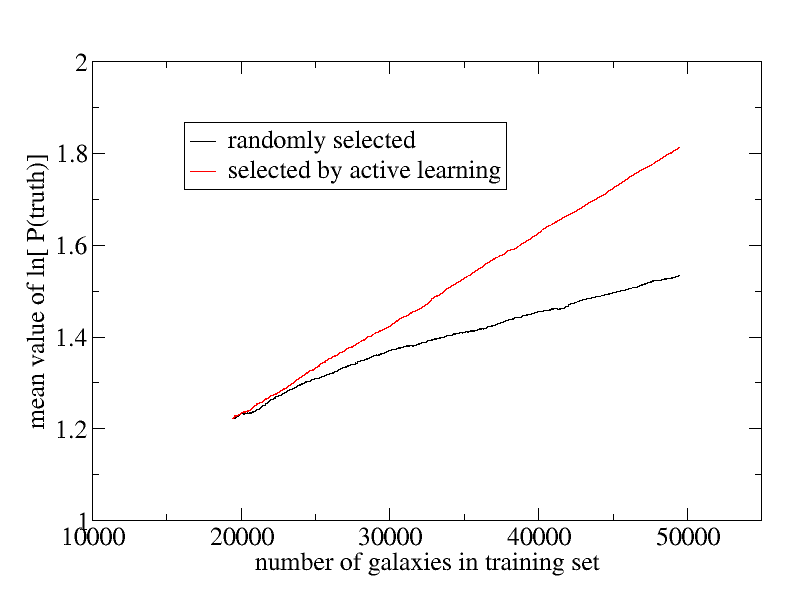
\includegraphics[scale=0.4]{learning_curve.png}
}
\caption{
Active learning applied to classification according to a scalar function on a
6-dimensional data space.  The horizontal axis is the size of the training data
set.  The vertical axis is the mean value of the output probability distribution
at the true value of the scalar function.  The black curve assembles the
training set randomly.  The red curve selects new training points that maximize
the figure of merit $\left(-\ln[P(\text{mode})]\right)$.
}
\label{fig:learning}
\end{figure}

In both empirical and forward-fitting photometric redshift codes, biases
arise from the fact that the distribution of training samples (templates)
is not the same in color and redshift space as the data the model will be
applied to.  Additional issues include the fact that some regions of color
space and some redshifts are more difficult to learn (require more training
samples).  We will show how our novel active learning algorithms can
achieve further improvements by choosing the most useful galaxies for
follow-up spectroscopy.

In a preliminary study we used a fully labeled data set containing galaxies
with both color measurements and true (spectroscopically determined)
redshift labels.  We simulated active learning by hiding the labels from
the GP learner and then providing them as requested by an active learning
algorithm.  We compared uniform random selection against uncertainty
sampling.  Figure \ref{fig:learning} demonstrates the results using the
problem presented in Figure \ref{fig:scatter}. %From a total of 97,000 data
%points, 
We start with 20,000 training points (consistent with the size of
current training sets used for photometric redshifts) and assess the efficacy of our
GP classifier by considering the mean value of $\ln[P(\text{truth})]$ as in
Figure \ref{fig:lnsum}.  Using this simplified active learning to add
to our training sample (as opposed to a random sampling strategy) 
leads to a significant improvement in the classifier's performance.

This study was done in a high signal-to-noise regime.  It takes no account
of the relative cost of doing one measurement or another.  No gaps exist in
the available training data.  These are all challenges that real-world
machine learning algorithms will face.  We will demonstrate our novel
methods on real data sets that contain all these additional challenges.


\section{Active Feature Acquisition:
Anomaly Detection and Classification in Massive Data
 Streams}


While the problem of photometric redshift determination is fertile ground for
the development of active learning algorithms, it poses little challenge for
active feature acquisition: for a given experiment, the photometric filters are
often immutable.  Fortunately, survey astronomy presents us with another 
problem, the identification and classification of transient sources,
which raises both the questions ``which objects should we
follow-up?'' and ``what observations should we make of them?''
With timescales as short as seconds to hours we require the ability to
identify, classify and report any detection in time to allow for
follow-up observations before the initial outburst
fades. Identification and classification must, therefore, be
undertaken in almost real-time with probabilistic classifications that
incorporate our uncertainties about our classification together with
the ability for algorithms to learn based on a posteriori information
from earlier classifications. It must be able to predict what
additional information might be needed to improved (or exclude) the
likelihood of a given classification and to specify which parameters
led to the source being classified as anomalous. Small errors in the
identification and classification of these anomalous sources will
swamp any underlying signal. The LSST will detect 7.5x10$^8$ sources
{\bf every night}. Even for the most numerous transient events (SNe)
this corresponds to less than 10$^{-5}$ of the total number of sources
identified being transient. For the most energetic bursters the
magnitude of the challenge is 500-fold larger.  Algorithms for
identifying anomalies and variability must, therefore, be robust to
false positives and missing data and must account for the cadence in
how we sample the time domain, variations in the quality of the data
due to atmospheric conditions, changes in the performance of the
telescope and camera and the possibility that we observe sources at
different wavelengths at different times.


%The next generation of astrophysical surveys will visit the same
%region of sky many thousands of times. This opening of the temporal
%domain in astrophysics offers the potential to discover new classes of
%physical phenomena while coming with many associated computational
%challenges. Variability within the universe is believed to be present
%on time scales of seconds through to tens of years. The shortest time
%scales correspond to the explosion of the most massive stars within
%the universe which produce short but intense optical and gamma-ray
%flashes. These outbursts provide direct tests of General Relativity
%and of high energy physical processes (at energies far beyond those
%accessible on the Earth). For example the rate at which these events
%occur constrains the age at which the first stars within the universe
%came into being. Intermediate timescale variability comes in the form
%of supernovae (SNe) which detonate, brighten and then dim. These
%exploding stars are known to have a narrow range of intrinsic
%brightnesses; they act as standard candles that can be used to
%determine the rate at which the universe expands and thereby measure
%its mass and energy content \cite{perlmutter99}. 
%Longer time scale
%variablity (including variability due to the velocity of sources)
%comes from variations in the luminosity of acretion disks around black
%holes, the motion of stars throughout our Galaxy and the motion of
%asteroids within the local solar system. These...
%With surveys such as the LSST we will detect 250,000 SNe per year
%increasing the accuracy of measures of the energy content of the
%universe by an order of magnitude.
%




\begin{figure}
\centerline{
\subfigure[]{
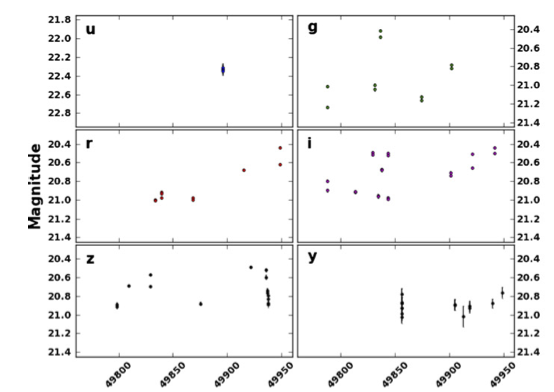
\includegraphics[scale=1.0]{becker_rrlyrae_uc.png}
\label{subfig:uc}
}
\subfigure[]{
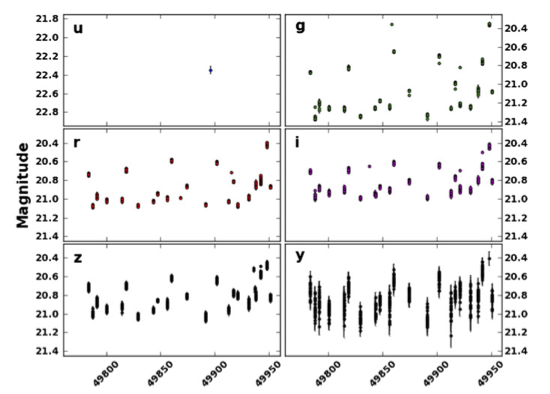
\includegraphics[scale=1.0]{becker_rrlyrae_dd.png}
\label{subfig:dd}
}
}
\centerline{
\subfigure[]{
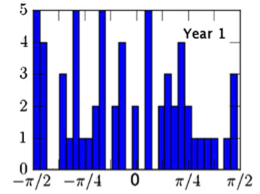
\includegraphics[scale=1.0]{becker_rrlyrae_year_1.png}
\label{subfig:year1}
}
\subfigure[]{
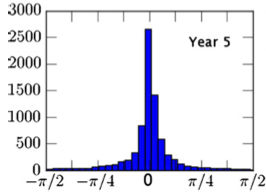
\includegraphics[scale=1.0]{becker_rrlyrae_year_5.png}
\label{subfig:year5}
}
}
\caption{
Taken from \cite{rrlyrae}.  Figure \ref{subfig:uc} shows the sampling of
a template RR Lyrae light curve at the LSST Universal Cadence.
Figure \ref{subfig:dd} shows the same for the 
Deep Drilling Cadence.  Figures \ref{subfig:year1} and \ref{subfig:year5} compare the scatter
in determining the phase of an RR Lyrae light curve after 1 year of Universal Cadence
data and 5 years of Universal Cadence data.  This illustrates the significant effect
on scientific output of more and more targeted data.
}
\label{fig:RRLyrae}
\end{figure}




\subsection{Active Learning for Transient Classification}


{\bf I have just copied-and-pasted the ``active learning for transients''
paragraphs from the previous draft}


Real-time automatic classification of objects is already widely acknowledged as a
necessary support technology for the forthcoming age of survey astronomy
\cite{djorgovski2011,richards2011,richards2012,graham2012,mahabal2008a,mahabal2011a}.
Objects will need to be categorized into known science classes so that novel
or rare objects can be flagged for detailed follow-up observations.
For transient events, algorithms must be able to make rapid
decisions so that sources can be targeted for follow-up 
and classifications learned before
objects return to their quiescent phases.  

A great deal of work has
already been done developing algorithms that can learn the classification of an
object given a fixed set of observations and training data.  
Mahabal {\it et al}. (2008a,2011a,2011b) propose to break down the
observations of a given object into $\{\Delta m,\Delta t\}$ pairs (where $m$
is magnitude and $t$ is time) and use the density of observations in this 
two-dimensional space as the basis for a Bayesian classification algorithm.
Mahabal {\it et al}. (2008b) alternatively propose to use those same 
$\{\Delta m,\Delta t\}$ pairs as the input to a GP regression
by which they will reconstruct the object's entire light curve as a function
of time, and then classify the object based on that reconstruction.
Anomaly detection has been attempted by decomposing light curves into
basis functions of different timescales and looking for events that occur
more rapidly than some fit baseline \cite{preston2009,blocker2013}.
Richards {\it et al}. (2011) use observations of transient objects to extract
periodic (e.g. the amplitude and frequency of the first two Fourier modes of
the object's light curve) and non-periodic (e.g. the variance and skewness of
all of the magnitude observations taken, regardless of their separation in
time) and feed those features into several tree-based classifiers.
They find misclassification rates lower than 30\% with their best method yielding a
misclassification rate of 22.8\%.  Using only non-periodic features, which will be
especially easy for survey telescopes to gather, rather than
full light curves, they 
find a misclassification rate of
between 26\% and 28\%.
Bloom {\it et al}. (2011) also use a tree-based automatic classifier on
Palomar Transient Factory data and find a 3.8\% error rate when
discriminating between four major classifications.  Richards {\it et al}.
consider a more complete set of 25 possible classifications.
Clearly, many possibile approaches are available for the automated
classification of transient objects, and not all of them rely upon highly
detailed observations to function.  
None of the above algorithms, however, make
any promises regarding their ability to deliver rapid recommendations for
optimum follow-up observations in real time.  This will be a significant
contribution to all time-sensitive sciences.

Similarly, a large number of classifiers have been developed which are optimized
for the case of binary classifications: ``Is something a quasar, or is it not?''
\cite{kim2011,pichara2012}, ``Is an object at redshift greater than 4 or is it
not?'' \cite{morgan2011}, ``Is an object a real astrophysical transient, or is
it an instrumental artifact?'' \cite{brink2012}.  The methods developed
(Random Forests; Support Vector Machiens; etc.) are all useful
and provide guidance for what can and should be attempted, however, they do not
deliver the robust, probabilistic, multi-class identifiers that will be required
by the rapid, big-data experiments of the next decades.

\subsection{Active Feature Acquisition and Active Search
for Transient Classification}

The input features for transient object classification will be 
a variable combination photometric
and morphologic measures taken at different increments in time.  The output
is a categorical variable indicating the class.
Brink {\it et al}. (2012) and Richards {\it et al}. (2012b) consider this
diversity of features in designing automatic classifiers on static data sets. 
They use cross-validation to
find that some features are more useful than others and that the inclusion
of all features degrades the performance of their classifier (see Figure 4 of
both references).  This
determination of optimal inputs is at the heart of active feature
acquisition.  Our
intention is to introduce an information-theoretical approach 
based on the output covariance matrix of equation \ref{eq:cov} which will allow
us to perform a similar determination in real time as observations are made,
directing experiments as they are performed.
We will not choose our follow-up observations based on cross-validation testing,
but rather based on which observations we expect to yield the most significant
decreases in the entropy of our probabilistic model.
An information-theoretical
approach has already been tried in the case of a static (i.e. off-line)
dataset by Huisje {\it et al}. 
(2011, 2012) who use a the correntropy as a measure of the
correlation between observed intensities at different time lags in already
observed light curves.  We will consider the effect on entropy of as-of-yet
untaken observations.  This will be a significant development towards the goal
of real-time object classification.

The active learning, active search, and active feature
acquisition choices for transient classification
all must be made in an online, streaming fashion.  
Rather than
considering an entire pool of test objects, they appear one at a time as
they are detected and the algorithm must decide whether and how to follow
up on each immediately as they are detected.  The culmination of our proposed
program of research will be to combine the methods devised above into a single
combined streaming algorithm as described below.

The three goals of active learning, active search, and active feature
acquisition will be combined
in a staged set of decisions.  When a new event or object is detected, the data
will be used to provide and estimated physical model for the object.
These models are the input variables for this object in the active
learning and active search algorithms.  In parallel, the active learning
and active search methods will decide whether to follow-up on this object.
If either of them selects the object, it is advanced to active feature
acquisition.  There additional observations on the object are selected and
the process for this object repeats.  An object that initially seemed
interesting to one algorithm may cease to be so after additional
observations or may be adopted by the other one.  The process for one
object terminates when neither active learning nor active search remains
interested in it or the object class and light curves are characterized
well enough that no more observations are required.

\section{Timeline and Development Plan}

We will focus on multiple projects in each of the four years of this
program.  Algorithms will be released as they are developed in a
twice-yearly release cycle.  Algorithm development will be undertaken using
data from current astronomical imaging surveys together with a series of
cosmological N-body simulations.  The time
dependent imaging data will be taken from the SDSS survey (including a 300
sq degree region observed 40+ times over the period of 10 years) and the
deep imaging data (to study the evolution of galaxies) from the Canada
France Legacy survey (CFHLS; \cite{hoekstra06}).

\noindent {\bf Year 1:} 

\begin{itemize}

\item Develop search based single-record and group-based anomaly detection
algorithms and apply them to single epoch SDSS data.  Anomalies identified
through this process will be released using an interface to Google Sky and
be based on the VOEvent protocols.

\item Develop sampling strategies for photometric redshift
 methods. Simulate the strategies and test them with different photometric
 redshift estimators.  Perform various cosmological analyses over the
 samples based on different sampling strategies, and estimate the
 sensitivity of the cosmological analyses to the details of the sampling
 strategies.

\end{itemize}

\noindent {\bf Year 2:} 

\begin{itemize}

\item Extend the anomaly detection algorithms to consider repeated
 observations of the same part of the sky.  We will analyze stellar
 sources where there are known populations with defined variability
 signatures (e.g.\ Cepheid variables) to provide validation for the
 analysis.  The algorithms will be applied to the larger SDSS data set to
 detect new time varying objects.

\item Improve classifiers for AGNs, asteroids, variable, and low mass stars
 based on using anomaly detection to identify mistakes and apply them to
 CFHLS and SDSS data.  We will implement an annotation service based on
 Galaxy Zoo to train the classifiers using labeled data.

\end{itemize}

\noindent {\bf Year 3:} 

\begin{itemize}

\item Develop search based systems modeling and apply it to characterizing
the relationship between measured attributes of stars and galaxies within
the SDSS data.

\item Develop and apply a search-based system for identifying differences
between simulations of galaxy evolution, observational data, and models
we learned from observations.

\item Based on the simulations for the optimal sampling, and our algorithms
 for machine learning for photometric redshifts, develop the next
 generation photometric redshift technique, apply it to emerging
 photometric peta-catalogs, and make the results publicly available.

\end{itemize}

\newpage





\begin{thebibliography}{99}

\bibitem[Abazajian {\it et al}. 2009]{Abazajian:2008wr}
  Abazajian, K.~N.{\it et al.}  [SDSS Collaboration]~2009,
  %``The Seventh Data Release of the Sloan Digital Sky Survey,''
  The Astrophysical Journal Supplement Series  {\bf 182}, 543
  [arXiv:0812.0649 [astro-ph]].
  %%CITATION = APJSA,182,543;%%

\bibitem[Abdalla {\it et al}. 2011]{abdalla}
Abdalla,~F.~B., Banerji,~M., Lahav,~O., and Rashkov,~V. 2011,
Monthly Notices of the Royal Astronomical Society {\bf 417}, 1891

\bibitem[Abramo {\it et al}. 2012]{narrow}
Abramo,~L.~R., Strauss,~M.~A., Lima,~M., Hern\'andez-Monteagudo,~C., Lazkoz,~R.,
Moles,~M., de Oliveira,~C.~M., Sendra,~I., Sodr\'e Jr.,~L., and
Storchi-Bergmann,~T. 2012, Monthly Notices of the Royal Astronomical Society
{\bf 423}, 3251

\bibitem[Albrecht {\it et al}. 2006]{detf}
Albrecht,~A., Bernstein,~B., Cahn,~R., Freedman,~W.~L., Hewitt,~J.,
Hu,~W., Huth,~J., Kamionkowski,~M., Kolb,~E., Knox,~L., Mather,~J.~C.,
Staggs,~S., Suntzeff,~N.~B. (Dark Energy Task Force) 2006,
``Report of the Dark Energy Task Force,''
\verb|http://jdem.gsfc.nasa.gov/science/DETF_Report.pdf|


\bibitem[Berg\'e {\it et al}. 2012]{psf}
Berg\'e,~J., Price,~S., Amara,~A., and Rhodes,~J. 2012,
Monthly Notices of the Royal Astronomical Society {\bf 419}, 2356

\bibitem[Blocker and Protopapas 2013]{blocker2013}
Blocker, Alexander W. and Protopapas, Pavlos 2013, arXiv:1301.3027

\bibitem[Bloom {\it et al}. 2011]{bloom2011}
Bloom,~J.~S., Richards,~J.~W., Nugent,~P.~E., Quimby,~R.~M., Kasliwal,~M.~M.,
Starr,~D.~L., Posnanski,~D., Ofek,~E.~O., Cenko,~S.~B., Butler,~N.~R.,
Kulkarni,~S.~R., Gal-Yam,~A., and Law,~N. 2011 [arXiv:1106.5491]

\bibitem[Bonfield {\it et al}. 2010]{bonfield}
Bonfield,~D.~G., Sun,~Y., Davey,~N., Jarvis,~M.~J., Abdalla,~F.~B.,
Banerji,~M., Adams,~R.~G. 2010, Monthly Notices of the Royal Astronomical Society 
{\bf 405} 987

\bibitem[Brammer {\it et al}. 2008]{eazy}
Brammer,~G.~B., van Dokkum,~P.~G., and Coppi,~P. 2008,
The Astrophysical Journal {\bf 686}, 1503

\bibitem[Brink {\it et al}. 2012]{brink2012}
Brink, Henrik, Richards, Joseph W., Poznanski, Dovi, Bloom, Joshua S., Rice,
John, Negahban, Sahand, and Wainwright, Martin 2012, arXiv:1209.3775

\bibitem[Bryan 2007]{brentsthesis}
Bryan, B., 2007, Ph.D. thesis
\verb|http://reports-archive.adm.cs.cmu.edu/anon/|
\verb|ml2007/abstracts/07-122.html|

\bibitem[Bryan {\it et al}. 2007]{bryan}
Bryan, B., Schneider, J., Miller, C.~J., Nichol, R.~C., Genovese, C., and
Wasserman, L., 2007,
The Astrophysical Journal {\bf 665}, 25

\bibitem[Budav\'ari 2008]{budavari2008}
Budav\'ari,~T. 2008 The Astrophysical Journal {\bf 695}, 747

\bibitem[Collister and Lahav 2004]{annz}
Collister,~A.~A. and Lahav,~O. 2004,
Publications of the Astronomical Society of the Pacific {\bf 116}, 345

\bibitem[Connolly {\it et al}. 2005]{imsim}
Connolly,~A.~J., Peterson,~J., Jernigan,~J.~G., Abel,~R., Bankert,~J.,
Chang,~C., Claver,~C.~F., Gibson,~R., Gilmore,~D.~K., Grace,~E., Jones,~R.~L.,
Ivezic,~Z., Jee,~J., Juric,~M., Kahn,~S.~M., Krabbendam,~V.~L., Krughoff,~S.,
Lorenz,~S., Pizagno,~J., Rasmussen,~A., Todd,~N. Tyson,~J.~A., and Young,~M.
2005, Society of the Photo-Optical Instrumentation Engineers (SPIE) Converence
Series {\bf 7738}, 53

\bibitem[Cunha {\it et al}. 2012]{cunha2012}
Cunha,~C.~E., Huterer,~D., Lin,~H., Busha,~M.~T., and Wechsler,~R.~H. 2012,
[arXiv:1207.3347]

\bibitem[Daniel and Linder 2010]{muvarpi2}
Daniel,~S.~F. and Linder,~E.~V. 2010, Physical Review D {\bf 82}, 103523

%\cite{Daniel:2011rr}
\bibitem[Daniel {\it et al}. 2011]{daniel2011} 
  Daniel,~S.~F., Connolly,~A.~J., Schneider,~J., Vanderplas,~J. and Xiong,~L. 
  %``Classification of Stellar Spectra with LLE,''
  The Astronomical Journal  {\bf 142}, 203 (2011)
  [arXiv:1110.4646 [astro-ph.SR]].
  %%CITATION = ARXIV:1110.4646;%%

\bibitem[Daniel {\it et al}. 2012]{daniel2012}
Daniel,~S.~F., Connolly,~A.~J., and Schneider,~J. 2012
[arXiv:1205.2708]

\bibitem[Das {\it et al}. 2011]{sudeep}
Das,~S., de Putter,~R., Linder,~E.~V., and Nakajima,~R. 2011,
[arXiv:1102.5090]

\bibitem[Davis {\it et al}. 2007]{essence}
Davis,~T.~M., M\"ortsell,~E., Sollerman,~J., Becker,~A.~C., Blondin,~S.,
Challis,~P., Clocchiatti,~A., Filippenko,~A.~V., Foley,~R.~J., Garnavich,~P.~M.,
Jha,~S., Krisciunas,~K., Kirshner,~R.~P., Leibundgut,~B., Li,~W., Matheson,~T.,
Miknaitis,~G., Pignata,~G., Rest,~A., Riess,~A.~G., Schmidt,~B.~P.,
Smith,~R.~C., Spyromilio,~J., Stubbs,~C.~W., Suntzeff,~N.~B., Tonry,~J.~L.,
Wood-Vasey,~W.~M., and Zenteno,~A. 2007, The Astrophysical Journal, {\bf 666},
716

\bibitem[de Putter {\it et al}. 2010]{roland}
de Putter,~R., Huterer,~D. and Linder,~E.~V. 2010, Physical Review D {\bf 81},
103513


\bibitem[Djorgovski {\it et al}. 2011]{djorgovski2011}
Djorgovski,~S.~J., Donalek,~C., Mahabal,~A.~A., Moghaddam,~B., Turmon,~M.,
Graham,~M.~J., Drake,~A.~J., Sharma,~N. and Chen,~Y. 2011
[arXiv:1110.4655] to appear in Statistical Analysis and Data Mining, ref. proc.
CIDU 2011 conf., eds. A. Srivastava and N. Chawla

\bibitem[Foster \it{et al}. 2009]{foster}
Foster, Leslie, Waagen, Alex, Aijaz, Nabeela, Hurley, Michael, Luis, Apolonio,
Rinsky, Joel, Satyavolu, Chandrika, Way, Michael J., Gazis, Paul, Srivastava,
Ashok 2009, Journal of Machine Learning Research {\bf 10} 857

\bibitem[Garnett {\it et al}. 2011]{Garnett11}
Garnett,~R., Krishnamurhty,~Y., Wang,~D., Schneider,~J., and Mann,~R. 2011,
``Bayesian Optimal Active Search on Graphs,'' KDD Workshop on Mining and
Learning with Graphs

\bibitem[Garnett {\it et al}. 2012a]{Garnett12}
Garnett,~R., Krishnamurthy,~Y., Xiong,~X., Schneider,~J., and Mann,~R. 2012a,
``Bayesian Optimal Active Search and Surveying,'' International Conference on
Machine Learning

\bibitem[Garnett {\it et al}. 2012b]{Garnett12a}
Garnett,~R., Ho,~S., and Schneider,~J. 2012b,
``Gaussian Processes for Identifying Damped Lyman-alpha Systems in Spectroscopic
Surveys,'' Neural Information Processing Systems 
workshop on Modern Nonparametric Methods in Machine Learning

\bibitem[Graham {\it et al}. 2012]{graham2012}
Graham,~M.~J., Djorgovski,~S.~G., Mahabal,~A., Donalek,~C., Drake,~A.,
Longo,~G. 2012 [arXiv:1208.2480] to appear in special issue of Distributed and
Parallel Databases on Data Intensive eScience

\bibitem[Huijse {\it et al}. 2011]{huijse2011}
Huijse, Pablo, Est\'evez, Pablo A., Zegers, Pablo, Pr\'incipe, Jose C.,
and Protopapas, Pavlos 2011, IEEE Signal Processing Letters {\bf 18}, 371

\bibitem[Huijse {\it et al}. 2012]{huijse2012}
Huijse, Pablo, Est\'evez, Pablo A., Protopapas, Pavlos, Zebers, Pablo,
and Pr\'incipe, Jos\'e C. 2012, arXiv:1212.2398

\bibitem[Huterer {\it et al}. 2006]{huterer2006}
Huterer,~D., Takada,~M., Bernstein,~G., and Jain,~B. 2006,
Monthly Notices of the Royal Astronomical Society {\bf 366}, 101

\bibitem[Kaufman {\it et al}. 2011]{kaufman}
Kaufman, Cari G., Bingham, Derek, Habib, Salman, Heitmann, Katrin, and Frieman,
Joshua A. 2011, The Annals of Applied Statistitcs {\bf 5} 2470

\bibitem[Kim {\it et al}. 2011]{kim2011}
Kim, Dae-Won, Protopapas, Pavlos, Byun, Young-Ik, Alcock, Charles, Khardon,
Roni, and Trichas, Markos 2011, arXiv:1101.3316

\bibitem[Kitching {\it et al}. 2008]{kitching}
Kitching,~T.~D., Taylor,~A.~N., and Heavens,~A.~F. 2008,
Monthly Notices of the Royal Astronomical Society {\bf 389} 173

\bibitem[Linder 2013]{linder2013}
Linder, Eric V. 2013, Journal of Cosmology and Astropartical Physics {\bf 1304}
031

\bibitem[Long {\it et al}. 2012]{long2012}
Long,~J.~P., El Karoui,~N., Rice,~J.~A., Richards,~J.~W., and Bloom,~J.~S. 2012,
Publications of the Astronomical Society of the Pacific {\bf 124} 280

\bibitem[LSST Collaboration 2011]{lsstoverview}
LSST Collaboration 2011, [arXiv:0805.2366]
\verb|http://www.lsst.org/lsst/overview/|

\bibitem[LSST Dark Energy Science Collaboration 2012]{desc}
LSST Dark Energy Science Collaboration 2012, [arXiv:1211.0310]

\bibitem[LSST Science Collaborations 2009]{sciencebook}
LSST Science Collaborations 2009, ``LSST Science Book'',
\verb|http://www.lsst.org/lsst/science/scibook|

\bibitem[Ma {\it et al}. 2006]{Ma2006}
Ma,~Z., Hu,~H., and Huterer,~D. 2006, The Astrophysical Journal {\bf 636}, 21

\bibitem[Ma {\it et al}. 2012]{YifeiMa12}
Ma,~Y., Garnett,~R., and Schneider,~J. 2012,
``Submodularity in Batch Active Learning and Survey Problems
on Gaussian Random Fields,''
Neural Information Processing Systems 
workshop on Discrete Optimization in Machine Learning

\bibitem[MacKay 1992]{mackay}
MacKay, David 1992, Neural Computation {\bf 4} 415

\bibitem[Mahabal {\it et al}. 2008a]{mahabal2008a}
Mahabal,~A., Djorgovski,~S.~G., Turmon,~M., Jewell,~J., Williams,~R.~R.,
Drake,~A.~J., Graham,~M.~G., Donalek,~C., Glikman,~E., and the Palomar-QUEST Team
2008a, Astronomische Nachrichten {\bf 329}, 288

\bibitem[Mahabal {\it et al}. 2008b]{mahabal2008b}
Mahabal,~A., Djorgovski,~S.~G., Williams,~R., Drake,~A., Donalek,~C.,
Graham,~M., Moghaddam,~B., Turmon,~M., Jewell,~J., Khosla,~A., and
Hensley,~B. 2008b [arXiv:0810.4527] to appear in proceedings fo the Class2008
conference (Classification and Discovery in Large Astronomical Surveys, Ringberg
Castle, 14-17 October 2008)

\bibitem[Mahabal {\it et al}. 2011a]{mahabal2011a}
Mahabal,~A.~A., Donalek,~C., Djorgovski,~S.~J., Drake,~A.~J.,
Graham,~M.~J., Williams,~R., Chen,~Y., Moghaddam,~B., and Turmon,~M.
2011a, [arxiv:1111.3699] to appear in Proc. IAU 285, ``New Horizons in Transient
Astronomy,'' Oxford, September 2011

\bibitem[Mahabal {\it et al}. 2011b]{mahabal2011b}
Mahabal,~A.~A., Djorgovski,~S.~G., Drake,~A.~J., Donalek~C., Graham,~M~J.,
Williams,~R.~D., Chen,~Y., Moghaddam,~B., Turmon,~M., Beshore,~E., and Larson,~S.
2011b, Bulletin of the Astronomical Society of India {\bf 39}, 387

\bibitem[Mandelbaum {\it et al}. 2008]{mandelbaum2008}
Mandelbaum,~R., Seljak,~U., Hirata,~C.~M., Bardelli,~S., Bolzonella,!M.,
Bongiorno,~A., Carollo,~M., Contini,~T., Cunha,~C.~E., Garilli,~B.,
Iovino,~A., Kambczyk,~P, Kneib,~J.-P., Knobel,~C., Koo,~D.~C., Lamareille,~F.,
Le F\`evre,~O., Leborgne,~J.-F., Lilly,~S.~J., Maier,~C., Mainieri,~V.,
Mignoli,~M., Newman,~J.~A., Oesch,~P.~A., Perez-Montero,~E., Ricciardelli,~E.,
Scodeggio,~M., Silverman,~J., and Tasca,~L. 2008, Monthly Notices of the Royal
Astronomical Society {\bf 386}, 781

\bibitem[McBride {\it et al}. 2011a]{mcbride2011a}
McBride,~C.~K., Connolly,~A.~J., Gardner,~J.~P., Scranton,~R., Newman,~J.~A.,
Scoccimarro,~R., Zehavi,~I., and Schneider,~D.~P. 2011a, The Astrophysical
Journal, {\bf 726}, 13

\bibitem[McBride {\it et al}. 2011b]{mcbride2011b}
McBride,~C.~K., Connolly,~A.~J., Gardner,~J.~P., Scranton,~R., Scoccimarro,~R.,
Berlind,~A.~A., Mar\'in,~F., and Schneider,~D.~P. 2011b, The Astrophysical
Journal {\bf 739}, 85

\bibitem[Moore {\it et al}. 2000]{Moore00}
Moore,~A., Connolly,~A., Genovese,~C., Grone,~L., Kanidoris,~N., Nichol,~R.,
Schneider,~J., Szalay,~A., Szapudi,~I., and Wasserman,~L. 2000,
``Fast Algorithms and Efficient Statistics: N-point Correlation Functions,'' in
MPA/MPE/ESO Conference on Mining the Sky [arXiv:astro-ph/0012333]

\bibitem[Morgan {\it et al}. 2011]{morgan2011}
Morgan, A.N., Long, James, Richards, Joseph W., Broderick, Tamara, Butler,
Nathaniel R., and Bloom, Joshua S. 2011, arXiv:1112.3654

\bibitem[Nakajima {\it et al}. 2012]{nakajima2011}
Nakajima,~R., Mandelbaum,~R., Seljak,~U., Cohn,~J.~D., Reyes,~R., and
Cool,~R. 2012, Monthly Notices of the Royal Astronomical Society {\bf 420}, 3240
[arXiv:1107.1395]

\bibitem[Nichol {\it et al}. 2006]{Nichol2006}
Nichol,~R.~C., Sheth,~R.~K., Suto,~Y., Gray,~A.~J., Kayo,~I., Wechsler,~R.~H.,
Marin,~F., Kulkarni,~G., Blanton,~M., Connolly,~A.~J., Gardner,~J.~P., Jain,~B.,
Miller,~C.~J., Moore,~A.~W., Pope,~A., Pun,~J., Schneider,~D., Schneider,~J.,
Szalay,~A., Szapudi,~I., Zehavi,~I., Bahcall,~N.~A., Csabai,~I., Brinkmann,~J.
2006, Monthly Notices of the Royal Astronomical Society {\bf 368}, 1507

\bibitem[Oluseyi {\it et al.} 2012]{rrlyrae}
Oluseyi, Hakeem M., Becker, Andrew C., Culliton, Christopher, Furqan, Muhammad,
Hoadley, Keri L., Regencia, Paul, Wells, Akeem J., Ivez\`ic, Zeljko, Jones, R.
Lynne, Krughoff, K. Simon, and Sesar, Branimir (2012), The Astronomical Joural
{\bf 144} 9

\bibitem[Pichara {\it et al}. 2012]{pichara2012}
Pichara, K., Protopapas, P., Kim, D.-W., Marquette, J.-B., and Tisserand, P.
2012, Monthly Notices of the Royal Astronomical Society, {\bf 427} 1284

\bibitem[Poczos and Schneider 2011]{poczos11alphadiv}
Poczos,~B. and Schneider,~J. 2011, ``On the Estimation of alpha-Divergences,''
Artificial Intelligence and Statistics (AISTATS)

\bibitem[Poczos {\it et al}. 2011]{Poczos2011UAI}
Poczos,~B., Xiong,~L., and Schneider,~J. 2011, ``Nonparametric Divergence Estimation with
Applications to Machine Learning on Distributions,''  Uncertainty in Artificial
Intelligence

\bibitem[Poczos {\it et al}. 2012]{poczos12CVPR}
Poczos,~B., Xiong,~L., Sutherland,~D., and Schneider,~J. 2012,
``Nonparametric Kernel Estimators for Image Classification,''
IEEE Conference on Computer Vision and Pattern Recognition

\bibitem[Preston {\it et al}. 2009]{preston2009}
Preston, Dan, Protopapas, Pavlos, and Brodely, Carla 2009, arXiv:0901.3329

\bibitem[Rasmussen and Williams 2006]{gp}
Rasmussen, C.~E. and Williams, C.~K.~I., 2006, ``Gaussian
Processes for Machine Learning''
\verb|http://www.GaussianProcess.org/gpml/|

\bibitem[Richards {\it et al}. 2004]{qso}
Richards,~G.~T., Nichols,~R.~C., Gray,~A.~G., Brunner,~R.~J., Lupton,~R.~H.,
Vanden Berk,~D.~E., Chong,~S.~S., Weinstein,~M.~A., Schneider,~D.~P.,
Anderson,~S.~F., Munn,~J.~A., Harris,~H.~C., Strauss,~M.~A., Fan,~X.,
Gunn,~J.~E., Ivezi\'c,~Z., York,~D.~G., Brinkmann,~J., and Moore,~A.~W. 2004,
The Astrophysical Journal Supplement Series, {\bf 155}, 257

\bibitem[Richards {\it et al}. 2011]{richards2011}
Richards,~J.~W., Starr,~D.~L., Butler,~N.~R., Bloom,~J.~S., Brewer,~J.~M.,
Crellin-Quick,~A., Higgins,~J., Kennedy,~R., and Rischard,~M. 2011,
The Astrophysical Journal {\bf 733}, 10

\bibitem[Richards {\it et al}. 2012a]{richards2012}
Richards,~J.~W., Starr,~D.~L., Brink,~H., Miller,~A.~A., Bloom,~J.~S.,
Butler,~N.~R., James,~J.~B., Long,~J.~P., and Rice,~J. 2012a
The Astrophysical Journal {\bf 744}, 192

\bibitem[Richards {\it et al}. 2012b]{richards2012b}
Richards, Joseph W., Starr, Dan L., Miller, Adam A., Bloom, Joshua S.,
Butler, Nathaniel R., Brink, Henrik, and Crellin-Quick, Arien 2012b,
The Astrophysical Journal Supplement Series {\bf 203} 32

\bibitem[Rosenfield {\it et al}. 2011]{rosenfield2011}
Rosenfield,~P., Connolly,~A., Fay,~J., Sayres,~C., and Tofflemire,~B. 2011,
Astronomical Society of the Pacific Conference Series {\bf 443}, 109

\bibitem[Scranton {\it et al}. 2002]{Scranton2002}
Scranton,~R., Johnston,~D., Dodelson,~S., Frieman,~J.~A., Connolly,~A.,
Eisenstein,~D.~J., Gunn,~J.~E., Hui,~L., Jain,~B., Kent,~S., Loveday,~J.,
Narayanan,~V., Nichol,~R.~C., O'Connell,~L., Soccimarro,~R., Sheth,~R.~K.,
Stebbins,~A., Strauss,~M.~A., Szalay,~A.~S., Sapudi,~I., Tegmark,~M.,
Vogeley,~M., Zehavi,~I., Annis,~J., Bahcall,~N.~A., Brinkman,~J., Csabai,~I.,
Hindsley,~R., Ivezic,~Z., Kim,~R.~S.~J., Knapp,~G.~R., Lamb,~D.~Q., Lee,~B.~C.,
Lupton,~R.~H., McKay,~T., Munn,~J., Peoples,~J., Pier,~J., Richards,~G.~T.,
Rockosi,~C., Schlegel,~D., Schneider,~D.~P., Stoughton,~C., Tucker,~D.~L.,
Yanny,~B., York,~D.~G. 2002, The Astrophysical Journal {\bf 579}, 48

\bibitem[Sesar {\it et al}. 2011]{linear}
Sesar,~B., Stuart,~J.~S., Ivezi\'c,~\u Z., Morgan,~D.~P., Becker,~A.~C., and
Wo\'zniak,~P. 2011, The Astronomical Journal {\bf 142}, 190

\bibitem[Settles 2009]{activelearning}
Settles,~B. 2009, ``Active Learning Literature Survey,'' Computer Sciences Technical
Report 1648, University of Wisconsin-Madison,
\verb|http://pages.cs.wisc.edu/~bsettles/active-learning/|


\bibitem[Shafieloo {\it et al}. 2012]{ericgp}
Shafieloo,~A., Kim,~A.~G., and Linder,~E.~V. 2012,
Physical Review D {\bf 85}, 123530 [arXiv:1204.2272]


\bibitem[Skibba {\it et al}. 2006]{Skibba2006}
Skibba,~R., Sheth,~R.~K., Connolly,~A.~J., and Scranton,~R. 2006,
Monthly Notices of the Royal Astronomical Society, {\bf 369}, 68

\bibitem[Straf 2003]{straf03}
Straf,~M.~L. 2003, Journal of the American Statistical Association {\bf 98}, 1

\bibitem[Szapudi {\it et al}. 2002]{Szapudi2002}
Szapud,~I., Frieman,~J.~A., Scoccimarro,~R., Szalay,~A.~S., Connolly,~A.~J.,
Dodelson,~S., Eisenstein,~D.~J., Gunn,~J.~E., Johnston,~D., Kent,~S.,
Loveday,~J., Meiksin,~A., Nichol,~R.~C., Scranton,~R., Stebbins,~A.,
Vogeley,~M.~S., Annis,~J., Bahcall,~N.~A., Brinkman,~J., Csabai,~I., Doi,~M.,
Fukigita,~M., Ivezi\'c,~\u Z., Kim,~R.~S.~J., Knapp,~G.~R., Lamb,~D.~Q.,
Lee,~B.~C., Lupton,~R.~H., McKay,~T.~A., Munn,~J., Peoples,~J., Pier,~J.,
Rockosi,~C., Schlegel,~D., Stoughtfon,~C., Tucker,~D.~L., Yanny,~B., York,~D.~G.
2002, The Astrophysical Journal {\bf 570}, 75

\bibitem[Vanderplas and Connolly 2009]{vdp2009}
Vanderplas,~J. and Connolly,~A.~J. 2009,
Astronomical Journal {\bf 138}, 1365

\bibitem[Wang {\it et al}. 2011]{wang2011}
Wang, Yuyang, Khardon, Roni, and Protopapas, Pavlos 2011
arXiv:1111.1315

\bibitem[Wang {\it et al}. 2012]{wang2012}
Wang, Yuyang, Khardon, Roni, and Protopapas, Pavlos 2012
arXiv:1203.0970

\bibitem[Wiley {\it et al}. 2011]{wiley2011}
Wiley,~K, Connolly,~A.~J., Gardner,~J., Krughoff,~S., Balazinska,~M., Howe,~B.,
Kwon,~Y., and Bu, ~Y. 2011, Publication of the Astronomical Society of the
Pacific {\bf 123}, 366

\bibitem[Xiong {\it et al}. 2011a]{Xiong2011gad}
Xiong,~L., Poczos,~B., Schneider,~J., Connolly,~A., Vanderplas,~J. 2011a,
``Hierarchical Probabilistic Models for Group Anomaly Detection,''
Artificial Intelligence and Statistics (AISTATS)

\bibitem[Xiong {\it et al}. 2011b]{xiong2011fgm}
Xiong,~L., Poczos,~B., and Schneider,~J. 2011, ``Group Anomaly Detection using Flexible
Genre Models,'' Neural Information Processing Systems

\bibitem[Yip {\it et al}. 2004]{yip2004a}
Yip,~C.~W., Connolly,~A.~J., Szalay,~A.~S., Budav\'ari,~T., SubbaRao,~M.,
Frieman,~J.~A., Nichol,~R.~C., Hopkins,~A.~M., York,~D.~G., Okamura,~S.,
Brinkmann,~J., Csabai,~I., Thakar,~A.~R., Fukugita,~M., 
and Ivezi\'c,~\u Z. 2004, The Astronomical Journal {\bf 128}, 585

\bibitem[Zhang and Schneider 2010a]{YiZhangICML2010}
Zhang,~Y. and Schneider,~J. 2010a, ``Projection Penalties: Dimension Reduction without
Loss,'' International Conference on Machine Learning

\bibitem[Zhang and Schneider 2010b]{YiZhangMultitask2010}
Zhang,~Y. and Schneider,~J. 2010b,
``Learning Multiple Tasks with a Sparse Matrix-Normal Penalty,''
Neural Information Processing Systems

\bibitem[Zhang {\it et al}. 2010]{YiZhangSDM2010}
Zhang,~Y., Schneider,~J., and Dubrawski,~A. 2010,
``Learning Compressible Models,'' Proceedings of SIAM Data Mining Conference

\bibitem[Zhang and Schneider 2011]{YiZhang2011multiECOC}
Zhang,~Y. and Schneider,~J 2011, ``Multi-label Output Codes using Canonical Correlation
Analysis,'' Artificial Intelligence and Statistics

\bibitem[Zhang and Schneider 2012]{YiZhang2012}
Zhang,~Y. and Schneider,~J. 2012, ``Maximum Margin Output Coding,''
International Conference on Machine Learning

\end{thebibliography} 
\label{lastpage}





\end{document}

\subsection{Active Learning and Photometric Redshifts}
\label{sec:mlpz}

The discussion above illustrates how the appropriate choice of machine
learning algorithm can affect the fidelity of one's photometric redshift
determinations.  Further gains can be made if one is similarly judicious in
choosing a training set.  While next generation surveys like the LSST will
be exclusively photometric, they will present us with large numbers of
galaxies which we will have the option to follow-up with off-site
spectroscopy.  It behooves us, therefore, to develop a quantitative way of
determining which galaxies represent the most effective use of these
limited follow-up resources.  Such methods fall in the field of active
learning and we will develop novel algorithms for this purpose.

Active learning algorithms iteratively decide which data points they will
collect outputs on and add to the training set.  The goal is to choose the
points that will most improve the model being learned.  At each step, they
consider the current training data, the potential training data that could
be collected, and the current learned model, and evalute each potential new
point according to some objective criterion.  After selecting one or more
new points, the outputs for those points are collected and added to the
training set and the process repeats.  The key to the active learning
algorithm is the specification of the objective criterion used for
selection.  Settles (2009) presents a survey of such criteria.



Real-time automatic classification of objects is already widely acknowledged as a
necessary support technology for the forthcoming age of survey astronomy
\cite{djorgovski2011,richards2011,richards2012,graham2012,mahabal2008a,mahabal2011a}.
Objects will need to be categorized into known science classes so that novel
or rare objects can be flagged for detailed follow-up observations.
For transient events, algorithms must be able to make rapid
decisions so that sources can be targeted for follow-up 
and classifications learned before
objects return to their quiescent phases.  A great deal of work has
already been done developing algorithms that can learn the classification of an
object given a fixed set of observations and training data.  
Mahabal {\it et al}. (2008a,2011a,2011b) propose to break down the
observations of a given object into $\{\Delta m,\Delta t\}$ pairs (where $m$
is magnitude and $t$ is time) and use the density of observations in this 
two-dimensional space as the basis for a Bayesian classification algorithm.
Mahabal {\it et al}. (2008b) alternatively propose to use those same 
$\{\Delta m,\Delta t\}$ pairs as the input to a Gaussian process regression
by which they will reconstruct the object's entire light curve as a function
of time, and then classify the object based on that reconstruction.
Richards {\it et al}. (2011) use observations of transient objects to extract
periodic (e.g. the amplitude and frequency of the first two Fourier modes of
the object's light curve) and non-periodic (e.g. the variance and skewness of
all of the magnitude observations taken, regardless of their separation in
time) and feed those features into several tree-based classifiers.
They find misclassification rates lower than 30\% with their best method yielding a
misclassification rate of 22.8\%.  Using only non-periodic features, which will be
especially easy for survey telescopes to gather, rather than
full light curves, they 
find a misclassification rate of
between 26\% and 28\%.
Bloom {\it et al}. (2011) also use a tree-based automatic classifier on
Palomar Transient Factory data and find a 3.8\% error rate when
discriminating between four major classifications.  Richards {\it et al}.
consider a more complete set of 25 possible classifications.
Clearly, many possibile approaches are available for the automated
classification of transient objects, and not all of them rely upon highly
detailed observations to function.

While significant attention has been paid to the problem of classifying an
object once training sets and observations have been assembled, relatively
little has been paid to optimizing the training set or observations.
Though the budgeted observing programs of survey telescopes leave little
time to follow-up serendipitous discoveries, other telescopes will be much
freer to fill in the gaps in survey-derived knowledge.  The question is
how best to do so.  The problem of sub-optimal training data is already being
faced by the community.  Figure 6 of Richards {\it et al}. (2011)
demonstrates that automated classifiers are much better at identifying
objects of common types, for which training data is abundant, than they are
at identifying objects of rare types, for which training data is sparse.
The authors address this problem in Richards {\it et al.} (2012a) by designing
an active learning algorithm which selectively adds to the training set,
choosing objects of uncertain classification and asking human classifiers to
provide detailed information (via either their expertise alone or with
follow-up observations) about the queried object.  They find that this scheme
reduces the misclassification rate 
of their classifier by approximately five percentage
points over a scheme which randomly constructs its training data set (see
their Figure 6).

This work demonstrates the potential of integrating active
learning into survey astronomy, however it does not 
account for the importance of
generating further 
observations about a source or the cost of these observations.  
The active learner implemented by
Richards {\it et al.} (2012a)
simply asks its human operators to provide classifications without offering
any guidance how.  Certainly, the humans would be almost guaranteed to
find the proper classification if they were to take both a full spectrum
and light curve of
the source, but this would come at the expense of a great deal of time and
effort.  We propose to eliminate this burden by using active learning not
only to designate objects to be added to the training set, but to designate
observations of those objects that would be the most efficient.  Figure 8 of
Richards {\it et al}. (2011) and Figure 13 of Bloom {\it et al}. (2011)
demonstrate that, for different classes of objects, different features are
more or less important.  If the machine learner already has an idea to what
class the queried object belongs, it should be able to give the operator a
recommendation of what observation to perform.  Maybe only a few color
measurments are needed to determine the object's physical origin.  
Maybe observations at only a few select epochs, rather than a drawn out time
series, will be needed to infer the object's complete light curve.
Maybe the required observations are consistent with the survey telescope's 
existing schedule, and no special follow-up will be required at all.  In this
way, active learning will allow us not only to maximize the science output of
our surveys, but to do so with the most efficient allocation of resources,
ensuring that we gain the most information about the most objects with the
least time and effort.

Active learning is integral to the identification and classification
of anomalies in cosmological data streams (e.g.\ through the
optimization of training sets used in classification).  Accomplishing this requires that we
expand the algorithms described previously to include active search,
and active feature acquisition. {\it Active feature acquisition}
entails deciding for each source, whether observations of additional
features (e.g.\ the colors of a source) would be valuable in
classifying an object.  Our recent work using Gaussian Process
(GP) regression shows that anomalous spectra can be inferred even 
from noisy input data (Garnett et al 2012). The key
advantage of this approach is that the GPs naturally provide a mean
and covariance for future unobserved parameters.  This uncertainty
propagates through to class labels and we can use it, for example, to
estimate the reduction in class uncertainty that will be gained by
observing a certain color at a given time.

In {\it active search} the ultimate objective in following up detected
anomalies is to maximize the number of interesting anomalies
classified and characterized while staying within a budget of
follow-up observations or experiments. The problem and the Bayesian
optimal algorithm for it are described in Garnett et al 2011 and Garnett
et al 2012a. We propose to expand on these approaches using scan
statistics to consider not just individual anomalies but also group
anomaly detection algorithms that consider arbitrary groupings of
self-similar anomalous records (Neil and Moore 2005).

Combining these approaches and adapting them to on-line or streaming
data (i.e.\ rather than considering an entire pool of test objects,
anomalies appear one at a time as they are detected and learning
algorithms must decide whether and how to follow up on each as they
are detected) we will address whether additional performance
improvements can be made through an integrated model and decision
algorithm. 

\noindent{\bf 4.\ Inference in the Presence of Noise and Gaps in a Data
  Stream:}
The final component of this research program will be the development
of a class of active learning methods that are robust to the presence
of noise and incomplete data. Even given the data volumes for the next
generation cosmological surveys their temporal sampling of the sky
will be poor (twice every three nights). Techniques such as GPs offer
two distinct advantages which render them particularly amenable to
integration into active learning frameworks.  Variance can be used
to assign an uncertainty to the predicted value and the covariance
provides the structure between all pairs of predicted and observed
outputs.  Bryan {et al} (2007) and Daniel {et al} (2012) use these
aspects to great affect, treating the determined variances as a
measure of the information that can be learned by promoting a query
point to a new training point and thus learning the likelihood surface
of a theory space with greater efficiency than traditional MCMC
methods.

The second advantage of Gaussian processes is their indifference to
the physical meaning of the inputs and outputs.  There is nothing
(other than computational cost) to prevent us from adding arbitrary
sets of variables and including them into the covariance
structure. This generalization makes them broadly applicable to a wide
range of experimental data. Indeed, Gaussian processes allow us to
incorporate any measured attribute (e.g.\ morphology, nearest-neighbor
distance) of our sources in a principled manner and use those
attributes to control the spread and bias in our estimation
techniques. In such a way, we can incorporate the measurement
uncertainties in our photometric colors and propagate them
consistently through to uncertainties in the determined photometric
redshifts. We propose to expand upon these directions to consider the impact
of not just measurement uncertainties but also missing data in terms
of characterizing the covariance.





\noindent
\begin{tabular}{ll}
{\bf Applicant/institution: } & University of Washington\\
{\bf Street Address: } & \\
{\bf Principal Investigator: } &Andrew Connolly \\
{\bf Telephone number: } & (206) 543 9541 \\
{\bf Email: } & ajc@astro.washington.edu \\
{\bf Administrative POC name, number, email:} & \\
{\bf Funding Opportunity FOA Number:} & DE-FOA-0000918 \\
{\bf DOE/OSP Office: } & Office of Advanced Scientific Computing Research \\
{\bf DOE/Technical Contact: } & Dr. Alexandra Landsberg \\
{\bf PAMS Preproposal tracking number: } & PRE-0000002147 \\
\end{tabular}

% \noindent 
% \begin{tabular}{ll}
% {\bf Applicant/institution: } & Carnegie Mellon University \\
% {\bf Street Address: } & 5000 Forbes Ave, Pittsburgh, PA  15213 \\
% {\bf Co-Principal Investigator: } & Jeff Schneider \\
% {\bf Telephone number: } & (412) 268 2339 \\
% {\bf Email: } & schneide@cs.cmu.edu \\
% {\bf Administrative POC name, number, email:} Kristen Jackson, (412) 268 9527, kristenr@andrew.cmu.edu & \\
% {\bf Funding Opportunity FOA Number:} & DE-FOA-0000918 \\
% {\bf DOE/OSP Office: } & Office of Advanced Scientific Computing Research \\
% {\bf DOE/Technical Contact: } & Dr. Alexandra Landsberg \\
% {\bf PAMS Preproposal tracking number: } & PRE-0000002147 \\
% \end{tabular}

\newpage

{\bf Collaborating Institutions:} \\
University of Washington, PI Andrew Connolly \\
Carnegie Mellon University, PI Jeff Schneider \\

{\bf Lead PI:} Andrew Connolly \\

\noindent
\begin{tabular}{|l|l|l|r|r|r|r|}
\hline
\multicolumn{7}{|c|}{\bf Learning in an Era of Uncertainty} \\ \hline
&       &             & Year 1 & Year 2 & Year 3 & Total \\
& Names & Institution & Budget & Budget & Budget & Budget \\ \hline
Lead PI & Andrew Connolly & U Washington & \$170K & \$170K & \$170K & \$510K \\ \hline
Co-PI & Jeff Schneider & Carnegie Mellon U & \$170K & \$170K & \$170K & \$510K \\ \hline
{TOTALS} & & & \$340K & \$340K & \$340K & \$1020K \\ \hline
\end{tabular}

% \label{firstpage}

% \maketitle 
\newpage

\begin{center}
{\bf \Large Learning in an Era of Uncertainty}
\end{center}

\section{Introduction:}
A new generation of DOE sponsored data intensive experiments and
surveys, designed to address fundamental questions in physics, materials, and
biology will come on-line over the next decade. These experiments
share many similar challenges in the fields of statistics and
machine-learning: how do we choose the next experiment or observation
to make in order that we maximize our scientific returns; how can we
identify anomalous sources (that may be indicative of new events or
potential systematics within our experiments) from a continuous stream
of data; how do we characterize and classify correlations and events
within data streams that are noisy and incomplete. The goal of this
proposal is to address these challenges through the development of a broad
class of novel and scalable machine-learning techniques centered
around the theme of active learning.

{\it Active learning} algorithms iteratively decide which data
points they will collect outputs on and add to a training set.  Their
goal is to choose the points that will most improves the model being
learned.  At each step, they consider the current training data, the
potential data that might be obtained, and the current learned model,
and evaluate what would be the best choice for the next observation,
experiment, or feature such that it improve the our knowledge of the
overall system (according to some objective criterion). The potential
impact of active learning algorithms is substantial (optimizing the
scientific returns from billion dollar investments in observational
facilities). To achieve these breakthroughs requires that we address
the challenge of how to scale active learning to the size and
complexity of the data expected from the next generation of
experiments.  For example, our inability to undertake a full look
ahead to the end of all possible experiments results in the
development of myopic heuristics that improve the speed of these
approaches but at a substantial cost in performance.  See, for example, 
Figure 1 from Garnett {\it et al}. (2011) and Figures
3 and 4 of Garnett {\it et al}. (2012a).

By addressing these challenges we propose to develop active learning
algorithms that will scale to data sets with hundreds of millions of
entries and petabytes of data. This work has the potential to impact
many of the data intensive sciences.. For this proposal, however, we
will focus our work in the context of DOE sponsored cosmology
experiments (i.e.\ the Dark Energy
Survey\footnote{http://www.darkenergysurvey.org}, and the Large
Synoptic Survey Telescope\footnote{http://www.lsst.org}). These
surveys are ideal proxies as their bandwidth (terabytes of data per
night and petabytes of data every couple of months) will enable high
precision studies of cosmology. The ability to use these data sets to
achieve an order of magnitude improvement in our constraints on our
understanding of cosmology and dark energy will, however, depend on
how well we can analyze, optimize, and calibrate data streams that are
inherently noisy and incomplete. This requires developing
fundamentally new approaches to the analysis of data at a scale,
speed, and complexity beyond the capabilities of current automated
machine learning methods.

\subsection{Project Objectives}
\label{sec:objectives}

We divide the problem of on-line big-data analysis into the following three
problems.

GPs :- Multimodal, missing data, scalability (matrix inversion), 

{\bf Active Learning.} Automatic regression and classification
algorithms require input from human experts against which to calibrate
themselves.  Often, the resources required to generate this input
(both in terms of human-hours and experimental apparatus) are
considerable.  We propose to develop algorithms to optimize the use of
these resources by determining what events' or objects' human
classification will maximize the improvement of the automatic
classifiers.  We have already implemented a toy version of such a
model on the problem of determing astronomical Doppler shifts (or
redshifts) using broad-band photometric data.  Our results (shown in
Figure \ref{fig:learning} below) give us hope that greater attention
will significantly increase the efficiency of future experiments.

{\bf Active Feature Acquisition.}  Active Learning selects specific
unknown events or objects for follow-up observation and classification
by human experts.  Active Feature Acquisition further refines our
inquiry by asking what kinds of follow-up observations will yield the
most information about the unknown object.  We propose to extend our
recent work on using Gaussian Processes (GPs) to detect damped
lyman-alpha (DLA) systems \cite{Garnett12a}.  In that work GP
regression was used on each observed, noisy spectrum to infer the
latent spectrum.  The single independent (input) variable was
wavelength.  In other problems (such as the identification of
astronomical transients) there will be several input variables which
we can choose to observe or ignore.  
We will build an information-theoretical framework to make this choice.
In the DLA work, a different
model was learned for spectra with and without a DLA.  DLAs were
classified by recognizing which model fit best.  In the proposed work,
we will learn a different model for each class of object and will
estimate class probabilities using Bayes rule for combining the prior
probability for each class and how well the respective models fit the
observations.  We will apply these techniques to the challenge of
characterizing the light curves of supernovae (used in measuring the
cosmic acceleration) from data with poor temporal sampling (i.e.\
increasing the number of supernovae that can be used for cosmological
experiments by an order of magnitude).  The key advantage of this
approach is that the GPs naturally provide a mean and covariance for
future unobserved observations.  This uncertainty propagates through
to class labels and we can use it to estimate the reduction in class
uncertainty that will be gained by observing a given observation at a
certain time.  The observation yielding the greatest reduction in
entropy for the class and the light curves for this object will be
taken.

{\bf Active Search.}  Often, the bulk of data yielded by any experiment will be
expected.  Ground-breaking research requires that we develop a method for
rapidly identifying and classifying novel events and objects
while staying within a
budget of follow-up observations.  This is an active search problem. The
problem and the Bayesian optimal algorithm for it are described in our
recent work \cite{Garnett11,Garnett12}.  As in active learning, the
acquisition of class labels is expensive and we need to learn a model to
predict these labels from limited input data.  However, the final
performance objective is not the accuracy of the classifier, but rather the
number of positives (i.e. objects from interesting classes)
identified. This previous work considered a binary classification problem: ``is
the object `interesting' or not?''  We will extend this work to allow for
classification according to a continuous scalar function and multiple discrete
classes.  We will design an algorithm that considers probability distributions
across all possible classes and how new observations will affect these
distributions with an eye towards reducing the entropy, or some other
information-theoretical measure of uncertainty.



% We
%propose to use the simple myopic algorithm described in that work.  It
%computes the probability of each point belonging to the positive class and
%chooses the largest.



%The active search and active learning algorithms each compute an objective
%criterion score for each object.  For photometric redshifts the scores are
%used to create a ranked list and observations are scheduled proceeding down
%the list.  When a budget is given for follow-ups on each batch of newly
%detected transients, going down a ranked list in each batch until that
%budget is exhausted is appropriate.

%However, when the budget is an aggregate over a longer time period a
%streaming decision on how much of the budget to spend on each batch must be
%made on that batch in isolation.  This will be done by choosing a score
%threshold.  The threshold will be set by evaluating the historical stream
%and setting it at a value that would yield a number of follow ups equal to
%an available budget for following up.  The threshold will be adjusted
%continuously as more observations are taken and the models and scientific
%goals change (e.g. the object types designated as ``interesting'' are
%changed).

Each of these goals will require us to develop algorithms to simultaneously
learn the latent physical model underlying a given data set, the uncertainties
around that model, and the potential information to be gained by futher studying
a specific instance of the model (an event or object as described above).
We believe that this problem can be best addressed by treating our models
non-parametrically and probabilistically, 
i.e. by solving for the probability distribution over the data's features.
For this reason, we propose to base our work on the formalism of Gaussian
Processes discussed in Section \ref{sec:gp} below.

\subsection{The Collaboration}

To accomplish the objectives laid out in this program we have
assembled a team experienced in algorithm design, data structures, and
in developing and delivering data mining algorithms that are actively
used by the cosmology community. The PIs of this research proposal
have a proven track record for propagating research ideas in
educational and multidisciplinary environments. Connolly and Schneider
have been part of an ongoing collaboration between machine learning,
cosmology and statistics for over a decade (noted by the President
of the American Statistical Association (ASA) as an exemplary
interdisciplinary research team \cite{straf03}).

Highlights from this collaboration include n-tree searching algorithms
that make the calculation of n-point correlation functions scale to
the size of current surveys \cite{GrayMoore} and that enable rapid
characterization of orbital tracks in sparsely sampled temporal data
\cite{kubica}. The software associated with these algorithms was made
publicly available and has been used to compute the 2--point function
on over 10$^6$ galaxies and the 3--point correlation function of
400,000 galaxies from the SDSS survey
\cite{Scranton2002,Szapudi2002,Nichol2006,mcbride2011a,mcbride2011b}
as well as in measures of the marked correlation functions
\cite{Skibba2006}.  As part of this collaboration \cite{yip2004a,
  vdp2009, daniel2011} introduced, to astrophysics, signal compression
and analysis techniques that are now regularly applied to the analysis
of spectroscopic surveys. More recently this collaboration has
developed algorithms to automatically classify astronomical objects
\cite{vdp2009,daniel2011} as well as an initial set of papers that use
a simplified active learning method to accelerate the exploration of
complex parameter spaces \cite{daniel2012}.  Schneider's group has led
the development of several new methods of regularization to learn
complex models with only a small amount of training data
\cite{YiZhangICML2010,YiZhangSDM2010,YiZhangMultitask2010,YiZhang2011multiECOC,YiZhang2012},
for non-parametric estimators for divergences and dependencies
\cite{poczos11alphadiv,Poczos2011UAI,poczos12CVPR}, and for graphical
models for finding groups of collectively anomalous records
\cite{Xiong2011gad,xiong2011fgm}.
 
Connolly leads the University of Washington data management group that
develops the algorithms and techniques for the real time analysis of
LSST data (including the real-time detection and characterization of
transients and anomalies).  Schneider heads a machine learning group
that has done extensive work on automatic anomaly detection and
pattern-recognition in complex data sets
\cite{Xiong2011gad,poczos12CVPR}.  Schneider, and Connolly are members
of the Large Synoptic Survey Telescope collaboration with Connolly the
software coordinator for the DOE sponsored Dark Energy Science
Collaboration (a collaboration of over 150 scientists working on the
characterization of dark energy).


On the educational front, all PIs have developed and taught computational techniques at the
graduate and undergraduate level including data-mining for
Astrophysics. Connolly recently completed a text book ``Statistics,
Data Mining, and Machine Learning in Astronomy: A Practical Python
Guide for the Analysis of Survey Data'' that will be published by
Princeton University Press and provides a comprehensive introduction
to the cutting-edge statistical methods together with the software
associated with these techniques. On sabbatical at Google, Connolly led the
development of Sky in Google Earth (aka Google Sky;
http://earth.google.com/sky), which was similarly successful at
engaging the public.

%We expect the proposed research to move beyond astrophysics to other
%data intensive sciences. In its broadest sense machine learning for
%massive Petabyte data archives drives many of the physical and
%biological sciences with catalogs containing hundreds millions of
%samples with thousands of measurements. The algorithms to be
%investigated here will also impact machine learning beyond their
%application to cosmology.  They move beyond the traditional learning
%of full models and are able to handle data that do not need to be
%pre-assembled into temporal sequences.  If successful, this will add
%new types of data sets and by inference new scientific fields to the
%list that can benefit from active learning of models.



\section{The Role of Active Learning in Cosmology}

Over the last decade a concordance model has emerged for the universe
that describes its energy content. The most significant contribution
to the energy budget today comes in the form of ``dark energy'', which
explains the observation that we reside in an accelerating
universe. Despite its importance to the formation and evolution of the
universe there is no compelling theory that explains the energy
density nor the properties of the dark energy. Understanding the
nature of dark energy remains as one of the most fundamental questions
in Physics today, impacting our understanding of cosmology, particle
physics, and potentially theories of gravity itself.  As noted in the draft
report of the Dark Energy Task Force (DETF; constituted jointly by
DOE, NSF and NASA), ``the nature of dark energy ranks among the very
most compelling of all outstanding problems in physical science''.


To address the question of the nature of dark energy a new generation
of DOE sponsored experiments are entering service (e.g.\ the Dark
Energy Survey, DES\footnote{http://www.darkenergysurvey.org} and the
Large Synoptic Sky Survey, LSST\footnote{http://www.lsst.org}).  These
surveys will represent a 40-fold increase in data rates over current
experiments (generating over 100 Petabytes of data over a period of 10
years) and decreasing the uncertainties on our measures of the
underlying properties of dark energy by more than a factor of ten.

Impact 

 On
these scales, statistical noise will no longer determine the accuracy
to which we can measure cosmological parameters. The control and
correction of systematics will ultimately determine our final
figure-of-merit. Prime amongst these systematics is the estimation of
distances to extragalactic sources, the identification of anomalous
events within the temporal universe (e.g.\ detecting optical flashes
and supernovae at cosmological distances), and the real time
classification of data in the presence of uncertainties and gaps
within the data stream.

With surveys such as the LSST we will detect 250,000 SNe per year
increasing the accuracy of measures of the energy content of the
universe by an order of magnitude.


more...

Describe multimodal error distributions, GMM, spanning the gap in
missing data, 
